\chapter{Implementación}

	\section{¿Qué es una FPAA?}
	Una FPAA  por sus siglas en inglés (Field Programmable Analog Arrays) es un dispositivo analógico equivalente a las FPGA (Field Programmable Garte Arrays). A diferencia de las FPGA que contienen una gran cantidad de módulos y conexiones que permiten configuraciones arbitrarias de lógica combinacional y secuencial, los FPAA generalmente contienen una pequeña cantidad de CABs (Configurable Analog Blocks). Los FPAA dirigidos al diseño analógico estándar generalmente presentan un CAB que contiene un amplificador operacional, un arreglo de capacitores programables, y ya sea un arreglo de resistencias programables para circuitos en tiempo continuo o switches configurables para circuitos de capacitores conmutados.
	Se trabajó con la tarjeta Anadigm QuadApex Develovment Boarsd v2.0 de la empresa Anadigm, la cual contiene 4 FPAAs AN231E04 que pueden conectarse en cadena y es programada mediante el software AnadigmDesigner2 (AD2). El diagrama esquemático de la tarjeta se puede ver en la Figura \ref{fig:esquematico_fpaa} del apéndice.
	
	\section{Características de la tarjeta y requerimientos}
	
		\subsection{Alimentación de la tarjeta}
	Para el correcto funcionamiento de la tarjeta, esta debe ser alimentada con una fuente de voltaje regulada a 5V de al menos 500mA conectada a la clema de dos terminales. La placa esta protegida contra la conexión de una fuente de voltaje con la polarización incorrecta. La tarjeta cuenta con un LED de color verde que indica que la placa se ha encendido correctamente. 
	
		\subsection{Instalación de drivers}

	No conecte la placa QuadApex v2.0 a la PC vía cable USB,  ni tampoco inicie AD2 ahora, el driver debe instalarse primero. Se asume que AD2 ya ha sido instalado y registrado en la computadora, de lo contrario entrar al link que aparece a continuación.

	Para instalar AD2 basta con acceder al siguiente link y seguir los pasos que muestra la pagina:

	\begin{center}
		\url{https://www.anadigm.com/sup_downloadcenter.asp?tab=ad2}
	\end{center}
	es recomendable guardar los datos de registro en un lugar seguro, al iniciar el programa por primera vez es necesario ingresar el \textbf{License ID} y la \textbf{License key}, estos estarán en el correo que le proporcionó a Anadigm. 

	El driver \textbf{CP210x\_{}Drivers.exe} está incluido en el AD2 CD o se puede encontrar en la página de Silicon Labs. Siga los siguientes pasos si es la primera vez que instala este driver, de lo contrario desinstale las versiones anteriores antes de continuar:

	\begin{enumerate}
		\item Ejecute como administrador el ejecutable  CP210x\_{}Drivers.exe. El destino por defecto del ejecutable es ‘‘C:\textbackslash{}Silabs\textbackslash{}Mcu\textbackslash{}CP210x’’.
		\item Para completar la instalación conecte la QuadApex v2.0 y enciéndala.
		\item Acceda al administrador de dispositivos y en \textbf{Puertos (COM y LPT)} asegúrese que el driver este bien configurado, si no aparece un signo de admiración y se le asigno un puerto COM  la instalación fue exitosa, de lo contrario dar clic derecho sobre el dispositivo y seleccionar \textbf{Actualizar controlador}, después buscar el  driver en la ruta del paso 1.
	\end{enumerate}
	el driver en este punto ya esta instalado. La instalación del driver y la asignación del puerto es necesaria solo una vez. Si se conecta subsecuentemente a otro puerto de USB de la PC puede ser necesario repetir el paso 3.

	
		\subsection{Jumpers por defecto}
	
	En la Tabla \ref{tab:jumpers} se muestra una lista con los jumpers que contiene la placa, una descripción de su funcionamiento y su posición por defecto. Es importante colocar la FPAA con todos sus jumper en el estado por defecto para entender secciones posteriores y evitar errores. La placa no contiene una cantidad muy grande de jumpers y usualmente solo se modificarán los jumpers J8,J9,J10, los cuales son los que controlan la cantidad de FPPAs activas.
	
\begin{table}[!ht]
		\centering
		\caption{Resumen de jumper de la placa.}
		\label{tab:jumpers}
		\resizebox{15cm}{!} {
		\begin{tabular}{|p{1.7cm}|p{9.5cm}|p{4.5cm}|p{5.5cm}|}
			\hline
			\textbf{Jumper} &  \textbf{Función} & \textbf{Estado por defecto}	& 	\textbf{Condición por defecto}\\
			\hline
			J1		&	Conecta la sección digital a la sección analógica.	&	Todos los 13 jumpers deben estar conectados &	Conecta completamente la alimentación, tierra y todas las señales digitales FPAA a la sección digital.\\
			\hline
			J2		&	Selecciona entre 16MHz y 40MHz para la fuente ACLK. &	Jumpers off &	ACLK$=$16MHz\\
			\hline
			J3		& Permite la descarga de la configuración de prueba a todos los FPAA desde FLASH (después de reiniciar o apagar y encender). El circuito de prueba despliega ondas sinusoidales a todas las salidas FPAA. &	Jumper off	& Descarga del circuito de prueba deshabilitado\\
			\hline
			J4		& Permite el almacenamiento de configuraciones primarias en el FLASH del PIC32 si el puente está activado. & Jumper off		&	No en modo de almacenamiento de configuraciones primarias.\\
			\hline
			J5		& Jumper de repuesto.	&	Jumper off &	-\\
			\hline
			J6		& Un jumper en J5 deshabilitará el módulo oscilador de 16MHz y tristateará su salida. Esto significa que el pin ACLK de los FPAA no se sincronizará, tampoco se sincronizará el microcontrolador PIC32, por lo que toda la placa se desactivará efectivamente. & Jumper off	& Oscilador de 16MHz habilitado	\\
			\hline
			J7		& Este jumper controla la generación de un suministro negativo (-3.3V) para las etapas del buffer de salida en la placa. El puente a la derecha desactiva el suministro negativo (lo ata al suelo). El puente a la izquierda permite el suministro.	& Jumper a la izquierda	&	Alimentación negativa habilitada\\
			\hline
			J8,9,10	& Estos jumpers en combinacion con ACT1, ACT2, ACT3, ACT4 controlan la cadena de FPAAs.	& Todos los jumpers especificados deben estar conectados	& Todas las FPAA en cadena	\\
			\hline
			J11		& Estos jumpers conectan el transceptor USB a la interfaz UART del microcontrolador PIC32. Si no se requiere control USB, estos 4 puentes se pueden quitar.	& Todos los jumpers conectados	& USB habilitado 	\\		
			\hline
		\end{tabular}
		}
\end{table}

		\subsection{Tamaño variable de cadena de FPAAs}

	La placa contiene 4 FPAAs en cadena. Esta cadena puede ser cortada a 3, 2 o 1, pero debe ser cortada deshabilitando FPAAs desde el final de la cadena (del lado derecho).

	\begin{itemize}
		\item Pare reducir la cadena a 3 FPAAs, remueva los jumpers de J10 y también el jumper marcado ACT4 de J1. Esto deshabilitará FPPAA \#4 (la más cercana a la fuente de alimentación.)
		\item Para reducir la cadena a 2 FPAAs, remueva los jumpers de J9 y J10 y también los jumpers marcados ACT3 y ACT4 de J1. Esto deshablitará los FPAAs \#3 y \#4.
		\item Para reducir la cadena a 1 FPAA, remueva los jumpers de J8, J9 y 10 y  también los jumpers marcados ACT2, ACT3 y ACT4 de J1. Esto deshabilitará los FPAA \#2, \#3 y \#4.
	\end{itemize}
	\textbf{Nota:} si se configura una cadena de FPAA y luego se desconectan 1 o más FPAA de la cadena, los FPAA desconectados aún mantendrán su configuración hasta que se reinicie la placa o se vuelva a configurar la cadena (reducida).

	\subsection{DIP Switches}
	
	El usuario puede hacer sus propias conexiones en la placa con cables, pero hay un conjunto de DIP switches que permiten una fácil conexión de ciertas rutas entre los FPAA vecinos y entre los FPAA y los input/output buffers. Estos interruptores están abiertos por defecto, lo que significa que todos están hacia la izquierda. El usuario puede cerrar los interruptores empujándolos hacia la derecha. En la Tabla \ref{tab:switches} se muestra un resumen de los switches. Los DIP switches son pequeños y del tipo deslizantes, por lo que se recomienda una herramienta afilada como un destornillador delgado para abrir y cerrar los switches. Algunos ejemplos se muestran a continuación:
	
	\begin{enumerate}
		\item Para conectar el filtro Rauch\_\#1\_IO1 a I1 de la FPPA\#{}1, cierre los 4 interruptores en S10.
		\item Para conectar O4 del FPAA\#{}1 a I1 del FPAA\#{}2, cierre los 2 interruptores superiores de S2.
		\item Para conectar O3 del FPAA\#{}1 al buffer de salida BUF\_\#1\_03, cierre ambos switches de S13.
	\end{enumerate}

	\begin{table}[!ht]
		\centering
		\begin{tabular}{|l|l|l|}
			\hline
			\textbf{Función} &  \textbf{Tipo} & \textbf{Labels}\\
			\hline
			Conectar filtros Rauch a entradas de FPAA 					& 4way 		& S8,9,10,11,15,16,17,18		\\
			\hline
			Conectar entre FPAAs 										& 4way 		& S2,3,4,5,6,7					\\
			\hline
			Conectar FPAA a buffers de salida 							& 2way 		& S12,13,14,19					\\
			\hline
		\end{tabular}
		\caption{DIP Switches}
		\label{tab:switches}
	\end{table}

		\subsection{Filtros Rauch y buffers de salida}
	
	La tarjeta cuenta con 2 buffers de entrada llamados filtros Rauch listos para usar, Rauch\_\#1\_I01 y Rauch\_\#2\_I01, estos son filtros multipropósito cuya su principal función es convertir una señal single-ended a una diferencial en la FPAA, internamente la FPAA trabaja únicamente con señales diferenciales y debido a esto el uso de estos filtros es imprescindibles para introducir señales externas, por ejemplo de generadores de funciones u otros circuitos. Si se usa una señal single-ended, es necesario conectar IN- a GND y conectar la señal en IN+.
	Para activar el filtro es necesario hacerlo desde el software AD2 haciendo doble clic en la IO cell apropiada (IOCell1-4), seleccionar Input y después Amplifier (Filter), esto es debido a que el filtro funciona en combinación con un amplificador integrado en la FPAA y los componentes pasivos de montaje superficial que vienen soldados de fabrica.
	
	Rauch\_\#1\_I01 está conectado a I/O1 de la FPAA \#1 y esta configurado con una frecuencia de corte muy alta ($F_{o} = 490$ kHz), una $Q = 0.707$ y ganancia unitaria. Los componentes pasivos que tiene son: $R_{1} = R_{2} = 22$k$\Omega$, $R_{3} = 10$k$\Omega$, $C_{1} = 22$pF y $C_{2} = 10$pF.  Rauch\_\#2\_I01 está conectado a I/O1 de la FPAA \#2 y esta configurado con una ganancia unitaria, una $Q = 0.707$ y una frecuencia de corte de poco más de 20 kHz, que es típica de una aplicación de audio. Los componentes pasivos respectivos son: $R_{1} = R_{2} = 470$k$\Omega$, $R_{3} = 220$k$\Omega$, $C_{1} = 22$pF y $C_{2} = 10$pF. Si se requiere una frecuencia de corte inferior o mayor, es muy fácil modificar este filtro sin quitar los componentes de montaje superficial debajo, simplemente agregando capacitores y resistencias TH. En la Figura \ref{fig:filtro_rauch} se muestra la representación esquemática del filtro Rauch y como se ve en AD2.
	
	\begin{figure}[!ht]
	\centering   
	\caption{Diferentes representaciones de filtro Rauch.}
	\label{fig:filtro_rauch}
		\begin{subfigure}{0.3\textwidth}
			\centering   
			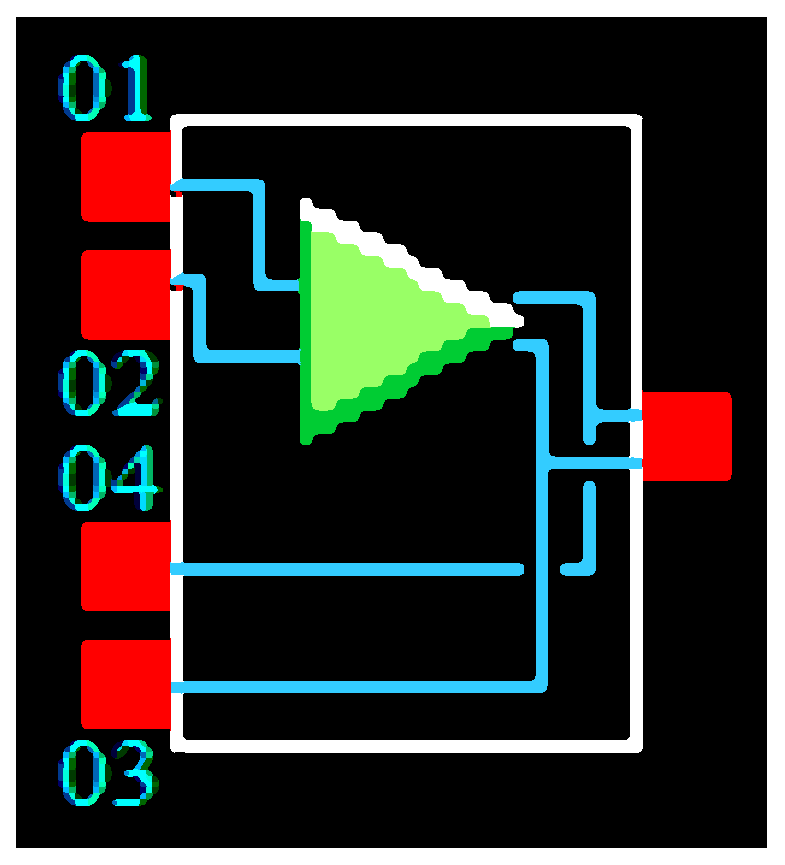
\includegraphics[width = 4cm]{V5_amplifier.eps}
			\caption{Vista en AD2.}
			\label{fig:V5_amplifier}
		\end{subfigure}
		\begin{subfigure}{0.65\textwidth}
			\centering   
			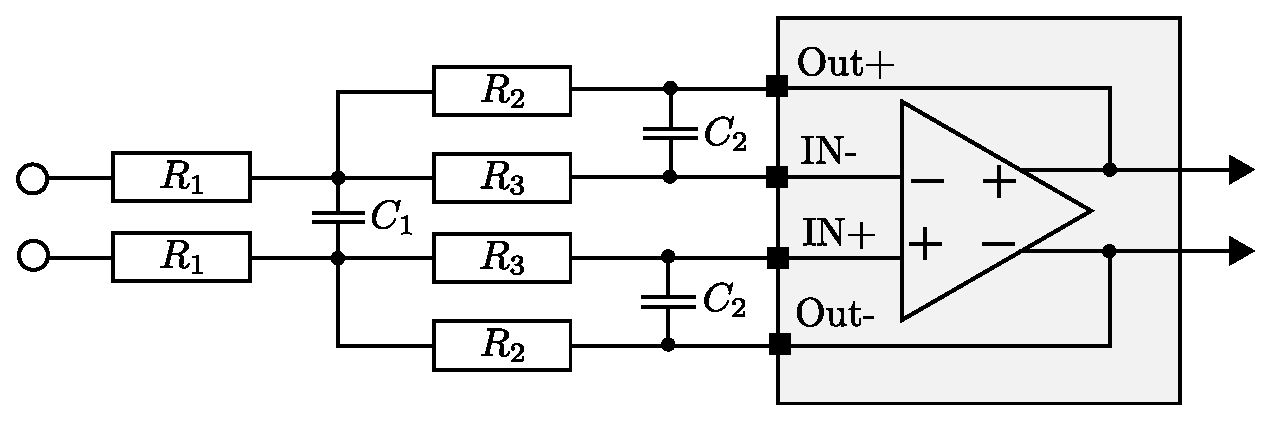
\includegraphics[width = 9.5cm]{V6_amplifier_esquematico.eps}
			\caption{Esquemático.}
			\label{fig:V6_amplifier_esquematico}
		\end{subfigure}
	\end{figure}

	Las siguientes ecuaciones sirven para calcular la ganancia, frecuencia de corte y factor de calidad $Q$ para cualquier filtro Rauch sobre la tarjeta:
	
	\begin{equation}
		G = \frac{R_{2}}{R_{1}}
	\end{equation}
	
	\begin{equation}
		F_{o} = \frac{1}{2 \pi R_{2}} \sqrt{ \frac{R_{1}+ R_{2} }{2 C_{1} C_{2} R_{1}}}
	\end{equation}
	
	\begin{equation}
		Q = \sqrt{\frac{C_{1} R_{1}}{2 C_{2} (R_{1} + R_{2})}}
	\end{equation}
	no obstante si se desea hacer el proceso inverso y determinar los valores de los componentes requeridos para una ganancia, frecuencia de corte y $Q$ especificadas, se pueden utilizar las siguientes ecuaciones: 
	
	\begin{equation}
		R_{2} = R_{1} G
	\end{equation}
	
	\begin{equation}
		R_{3} = \frac{R_{1} G}{G + 1}
	\end{equation}
	
	\begin{equation}
		C_{1} = \frac{Q (G + 1)}{2 \pi G F_{o} R_{1}}
	\end{equation}
	
	\begin{equation}
		C_{2} = \frac{1}{4 \pi G F_{o} Q R_{1}}
	\end{equation}
	consideremos el siguiente ejemplo representativo. Construya un filtro Rauch con las siguientes características: ganancia de 1.5, una frecuencia de corte $F_{o} = 20$ kHz y $Q = 0.707$. Utilizando las ecuaciones anteriores y proponiendo $R_{1} = 10$k$\Omega$ obtenemos:
	
	\vspace{-1cm}
	\begin{align*}
		R_{2}	&=	15\mathrm{k}\Omega		& C_{1}	&=	0.938\mathrm{nF} \approx	1\mathrm{nF}\\
		R_{3}	&=	6\mathrm{k}\Omega \approx	5.6\mathrm{k}\Omega		& C_{2}	&=	0.375\mathrm{nF} \approx	330\mathrm{pF}\\
	\end{align*}	
	
	\vspace{-1cm}
	La tarjeta también cuenta con 2 buffers de salida listos para usar, Buf\_\#1\_O3 y Buf\_\#2\_O3, cuyo principal propósito es convertir la salida diferencial de la FPAA a una single-end. 
	Buf\_\#1\_O3 está conectado a O3 de la FPAA \#1 y está configurado con una frecuencia de corte muy alta ($F_{o} = 480$ kHz) y una ganancia unitaria. Los componentes pasivos que tiene son: $R_{1} = R_{2} = 33$k$\Omega$, $C_{1} = 10$pF. Buf\_\#2\_O3 está conectado a O3 de FPAA \#2 y esta configurado con una ganancia unitaria y una frecuencia de corte de poco más de 20 kHz, que es típica de una aplicación de audio. Los componentes pasivos que tiene son: $R_{1} = R_{2} = 470$k$\Omega$, $C_{1} = 15$pF. Si se requiere una frecuencia de corte inferior o mayor, es muy fácil modificar este filtro sin quitar los componentes de montaje superficial debajo, simplemente agregando capacitores y resistencias TH. En la Figura \ref{fig:V7_buffer_esq} se muestra el diagrama esquemático del buffer de salida.
	\begin{figure}[!hbp] 
		\caption{Esquemático buffer de salida.}
		\label{fig:V7_buffer_esq}
		\centering
		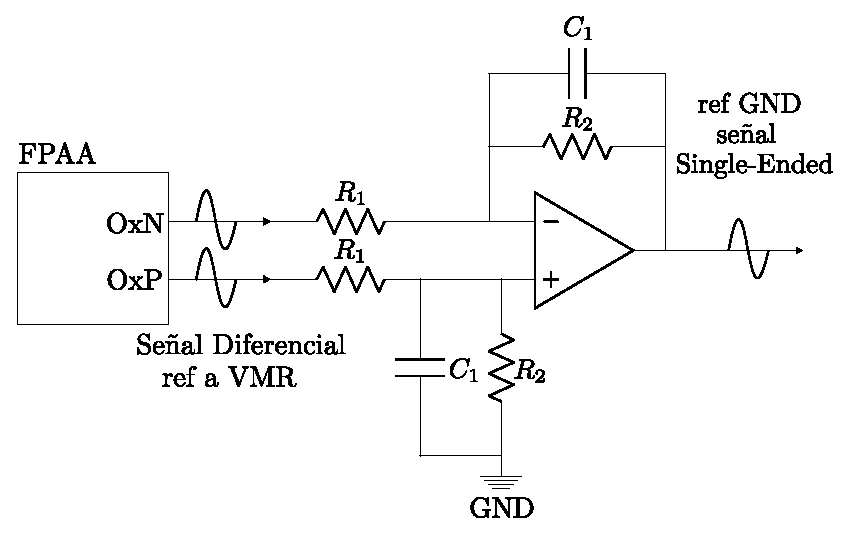
\includegraphics[width = 9cm]{V7_buffer_esq.eps}
	\end{figure}
	
	Las ecuaciones para calcular la ganancia y la frecuencia de corte de los buffers de salida son las siguientes:
	
	\begin{equation}
		G = \frac{R_{2}}{R_{1}}
	\end{equation}
	
	\begin{equation}
		F_{o} = \frac{1}{2 \pi R_{2} C_{1}}
	\end{equation}
	
	Es importante resaltar que para utilizar tanto los filtros Rauch como los buffers de salida sin cables adicionales es necesario cerrar los DIP switches correspondientes para hacer las conexiones sobre la tarjeta, sin embargo no hay que olvidar que siempre es posible cablear externamente utilizando jumpers desde los filtros a cualquiera de las entradas o salidas de las FPAA.
	
		\subsection{Circuito de prueba}

	La tarjeta es capaz de autoconfigurar los FPAA con un circuito de prueba para una verificación rápida de la placa. Para hacer esto, coloque un jumper en J3 y reinicie la tarjeta. Todos los FPAA en la cadena ahora se configurarán con el circuito de prueba (el LED verde indica que la configuración fue exitosa). Este circuito de prueba genera una onda sinusoidal en todas las 7 salidas del FPAA (14 salidas diferenciales). La frecuencia de esta onda sinusoidal es de 1 kHz en FPAA \#{}1, 2 kHz en FPAA \#{}2, 4 kHz en FPAA \#{}3 y 8 kHz en FPAA \#{}4. Si se habilitan menos de 4 FPAA en la cadena, solo se configurarán aquellos FPAA que estén habilitados. Si se coloca un jumper en J3 y J4, se cargará un circuito diferente en los FPAAs. Este es un circuito de prueba especial utilizado por Anadigm durante la producción. Se aconseja al usuario que no coloque jumpers en J3 y J4 al mismo tiempo.

	\section{AnadigmDesigner2}
	
	AD2 es un software creado por la empresa Anadigm el cual permite construir fácilmente circuitos analógicos complejos seleccionado, colocando y cableando juntos subcircuitos de bloques de construcción  denominados CAM (Configurable Analog Modules), estos aportan flexibilidad y sencillez en el proceso diseño debido a que son bloques que hacen desde funciones sencillas como inversores o comparadores hasta diseños completos como filtros y multiplicadores. Los CAM pueden interconectarse fácilmente unos con otros y únicamente necesitan pequeñas configuraciones para su correcto funcionamiento. Los circuitos analógicos que se construyen pueden ser descargados a la FPAA y esta funcionará como el circuito construido. Los resultados del diseño analógico pueden ser visto de inmediato utilizando un generador de funciones y un osciloscopio (hardware-in-the-loop). Los CAM más utilizados son los mostrados en la Tabla \ref{tab:CAMs_AD2}. En secciones posteriores se abordará con más detalle como configurarlos y cuales son las ecuaciones necesarias para calcular los parámetros de cada uno.  
	
	\begin{table}[!ht]
	  \centering
	  \caption{CAMs básicos de AD2.}
	  \label{tab:CAMs_AD2}
	  \begin{tabular}{>{\centering\arraybackslash}m{3cm} >{\centering\arraybackslash}m{5cm} >{\centering\arraybackslash}m{5cm}}
	    \hline
	    \textbf{Nombre} & \textbf{Función de transferencia} & \textbf{Descripción}\\ 
	    \hline
	    {\scriptsize \textbf{GainInv}}
	    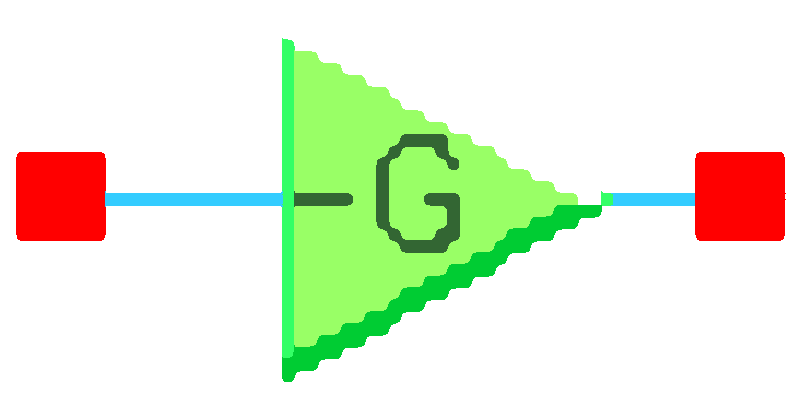
\includegraphics[width=2.2cm]{T7_Inversor.eps}
	    &
	      $\frac{V_{\mathrm{out}} (s)}{V_{\mathrm{in}}(s)} = - G$
	    & 
	      \begin{itemize}[leftmargin=0cm,noitemsep]
	      \begin{scriptsize}
			\item[] Ganancia inversora.
			\item[] Gain: 0.01 - 100.0 V/V
	      \end{scriptsize}
	      \end{itemize}
	    \\ %-------------------------------------------------------
	    {\scriptsize \textbf{Integrator}}
	    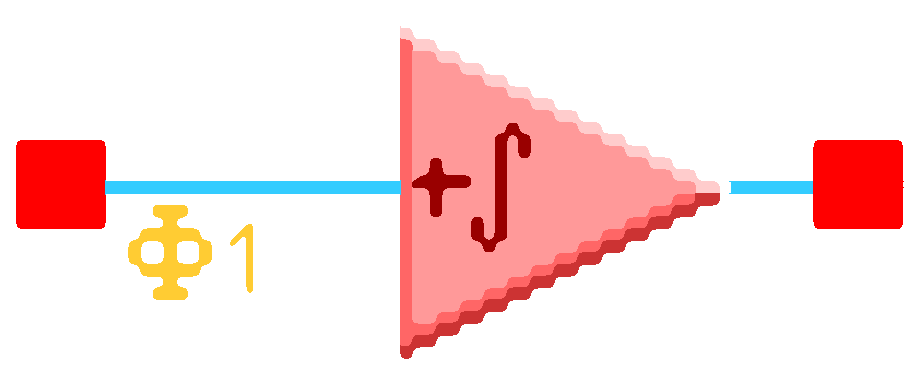
\includegraphics[width=2.5cm]{T1_Integrador.eps}
	    &
	      $ \frac{V_{\mathrm{out}} (s)}{V_{\mathrm{in}}(s)} = \frac{\pm K}{s}$
	    & 
	      \begin{itemize}[leftmargin=0cm,noitemsep]
	      \begin{scriptsize}
			\item[] Integrador con una constante de integración programable. La salida puede ser inversora o no inversora.
	      \end{scriptsize}
	      \end{itemize}
	    \\ %-------------------------------------------------------
	    {\scriptsize \textbf{Voltage}} \linebreak
	    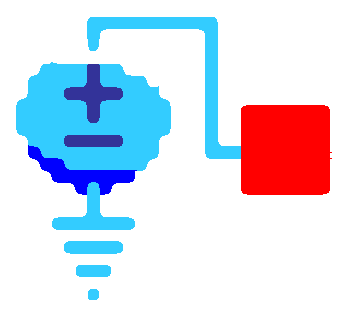
\includegraphics[width=1cm]{T6_DC_voltage.eps}
	    &
	      $V_{\mathrm{out}} = \pm 2$
	    & 
	      \begin{itemize}[leftmargin=0cm,noitemsep]
	      \begin{scriptsize}
			\item[] Referencia de voltaje de $\pm$ 2 V.
	      \end{scriptsize}
	      \end{itemize}
	    \\ %-------------------------------------------------------
	    {\scriptsize \textbf{TransferFunction}} \linebreak
	    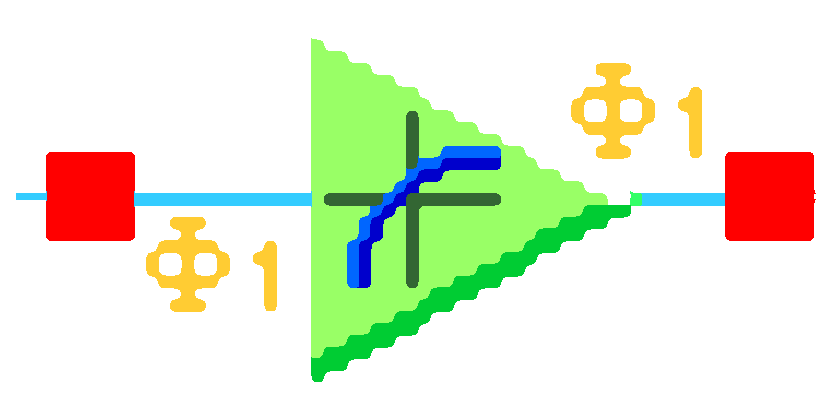
\includegraphics[width=2.5cm]{T3_Transferfunction.eps}
	    &
	    & 
	      \begin{itemize}[leftmargin=0cm,noitemsep]
	      \begin{scriptsize}
			\item[] \textbf{Lookup Table}: función de transferencia especificada por el usuario de 256 de pasos de cuantificación.  
	      \end{scriptsize}
	      \end{itemize}
	    \\ %-------------------------------------------------------
	    {\scriptsize \textbf{Multiplier}} \linebreak
	    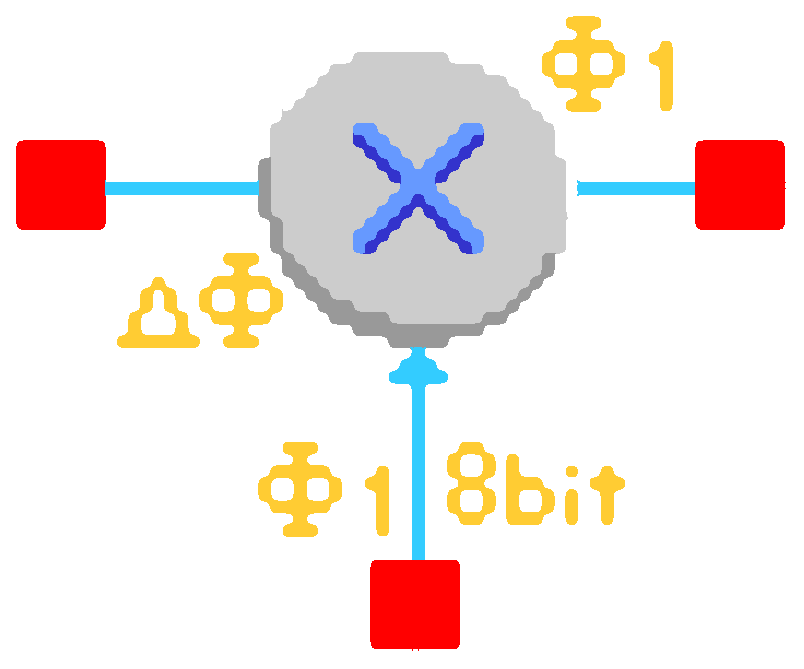
\includegraphics[width=2.5cm]{T2_Multiplicador.eps}
	    &
	      $V_{\mathrm{out}} = M \cdot V_{x} \cdot V_{y}$
	    & 
	      \begin{itemize}[leftmargin=0cm,noitemsep]
	      \begin{scriptsize}
			\item[] $V_{x}$ es la entrada de voltaje izquierda.
			\item[] $V_{y}$ es la entrada de voltaje inferior cuantificado de 8 bits.
			\vspace{-0.15cm}
			\item[] $M$ factor de multiplicación.
	      \end{scriptsize}
	      \end{itemize}
	   \\ %-------------------------------------------------------
	    {\scriptsize \textbf{SumInv}} \linebreak
	    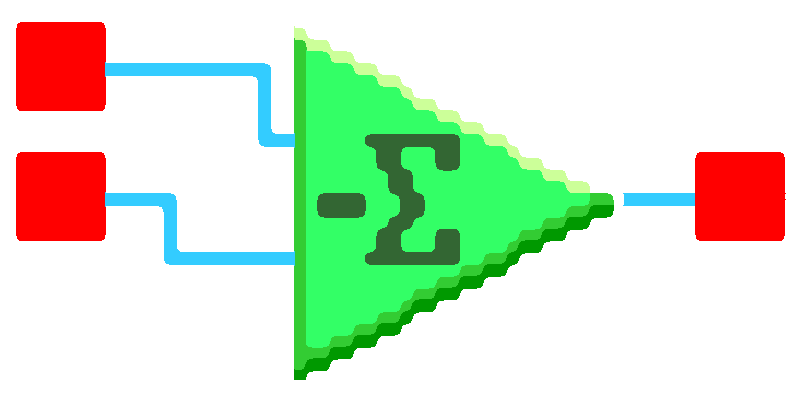
\includegraphics[width=2.5cm]{T0_Sumador_Inv.eps}
	    &
	      \begin{footnotesize}
	      	$V_{\mathrm{out}} = - G_{1} V_{\mathrm{in1}} - G_{2} V_{\mathrm{in2}} - G_{3} V_{\mathrm{in3}}$
	      \end{footnotesize}
	    & 
	      \begin{itemize}[leftmargin=0cm,noitemsep]
	      \begin{scriptsize}
			\item[] Configurable desde 2 hasta 3 entradas.
			\item[]	Cada entrada tiene una ganancia programable.
			\vspace{-0.15cm}
			\item[] Configurable desde 2 hasta 4 entradas. 
	      \end{scriptsize}
	      \end{itemize}
	    \\ %-------------------------------------------------------
	    {\scriptsize \textbf{SumDiff}} \linebreak
	    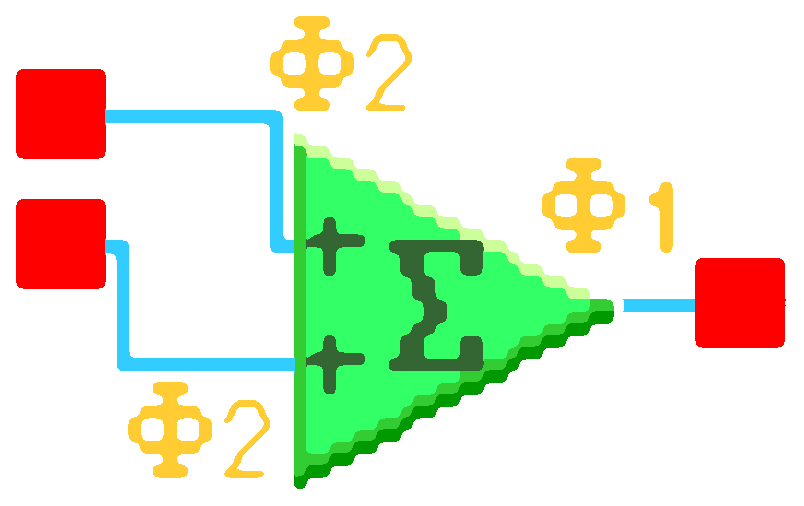
\includegraphics[width=2.5cm]{T8_Sumador.eps}
	    &
	      \begin{footnotesize}
	      	$V_{\mathrm{out}} = \pm G_{1} V_{\mathrm{in1}} \pm G_{2} V_{\mathrm{in2}} \pm G_{3} V_{\mathrm{in3}} \pm G_{4} V_{\mathrm{in4}}$
	      \end{footnotesize}
	    & 
	      \begin{itemize}[leftmargin=0cm,noitemsep]
	      \begin{scriptsize}
			\item[] Las entradas pueden ser inversoras o no inversoras.
			\item[]	Cada entrada tiene una ganancia programable.
			\vspace{-0.15cm}
			\item[] Configurable desde 2 hasta 4 entradas. 
	      \end{scriptsize}
	      \end{itemize}
	    \\ %-------------------------------------------------------
	    {\scriptsize \textbf{FilterBilinear}} \linebreak
	    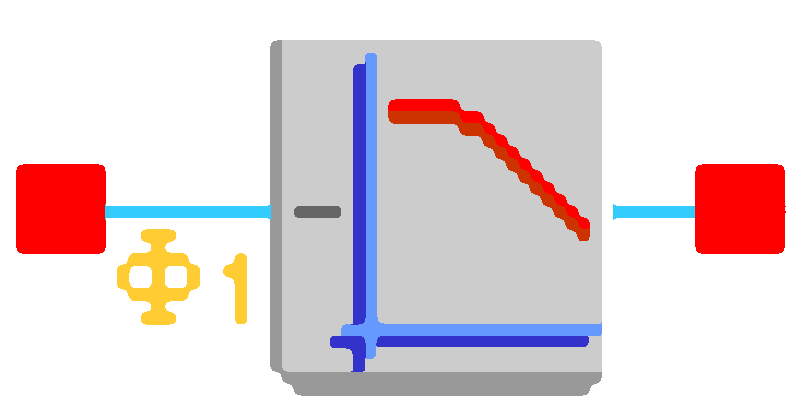
\includegraphics[width=2.5cm]{T9_FilterBilinear.eps}
	    &
	      \begin{scriptsize}
			 \textbf{Low Pass Bilinear Filter} \linebreak
	      	 $\frac{V_{\mathrm{out}}(s)}{V_{\mathrm{in}}(s)} = \pm \frac{2 \pi f_{0} G}{s + 2 \pi f_{0}}$ \linebreak
	      	 \textbf{High Pass Bilinear Filter} \linebreak
	      	 $\frac{V_{\mathrm{out}}(s)}{V_{\mathrm{in}}(s)} = - \frac{Gs}{s + 2 \pi f_{0}}$ \linebreak
	      	 $\vdots$
	      \end{scriptsize}
	    & 
	      \begin{itemize}[leftmargin=0cm,noitemsep]
	      \begin{scriptsize}
			\item[] Puede ser configurado como pasabajas, pasaaltas, pasatodas o general (Polo y cero).
	      \end{scriptsize}
	      \end{itemize}
	    \\ %-------------------------------------------------------
	    {\scriptsize \textbf{FilterBiquad}} \linebreak
	    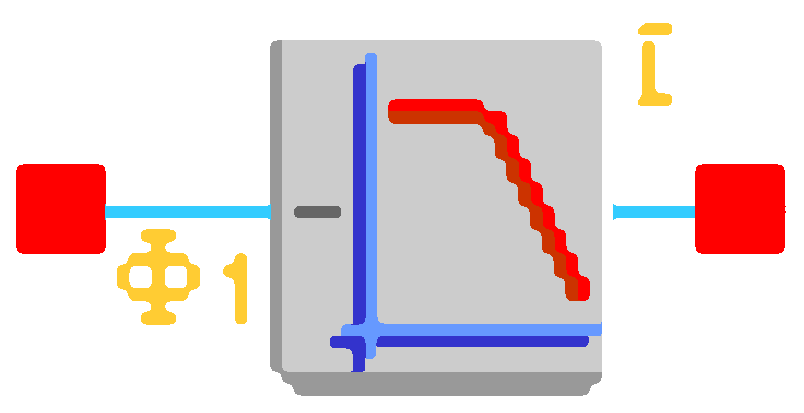
\includegraphics[width=2.5cm]{T10_FilterBiquad.eps}
	    &
	      \begin{scriptsize}
			 \textbf{Low Pass Biquadratic Filter} \linebreak
	      	 $\frac{V_{\mathrm{out}}(s)}{V_{\mathrm{in}}(s)} = \frac{\pm 4 \pi^{2} f_{0}^{2} G}{s^{2} + \frac{2 \pi f_{0}}{Q}s + 4 \pi^{2} f_{0}^{2}}$ \linebreak
	      	 \textbf{High Pass Biquadratic Filter} \linebreak
	      	 $\frac{V_{\mathrm{out}}(s)}{V_{\mathrm{in}}(s)} = \frac{-G s^{2}}{s^{2} + \frac{2 \pi f_{0}}{Q} s + 4 \pi^{2} f_{0}^{2}}$ \linebreak
	      	 $\vdots$
	      \end{scriptsize}
	    & 
	      \begin{itemize}[leftmargin=0cm,noitemsep]
	      \begin{scriptsize}
			\item[] Puede ser configurado como pasabajas, pasaaltas, pasabanda, rechazabanda o general (Polos y ceros).
	      \end{scriptsize}
	      \end{itemize}
	    \\ %-------------------------------------------------------
	    \hline
	  \end{tabular}
	\end{table}
	
		\subsection{Comunicación con AD2}

	Para este punto la tarjeta ya puede ser programada lo que en este caso significa configurar los FPAA. Esto puede realizarse desde una PC o una laptop usando un cable estándar USB tipo A-B. La tarjeta usa una emulación de comunicación serial de tal manera que desde la computadora la tarjeta aparecerá como un puerto COM.

	Para programar la tarjeta el primer paso consiste en asegurarse de seleccionar la tarjeta adecuada y comprobar que esta funcione correctamente, para esto, conecte el cable USB entre la placa y la computadora y encienda la tarjeta. Abra AD2 y haga clic en \textbf{Settings/Preferences}, en la pestaña \textbf{Chip} seleccione \textbf{AN231E04}, después diríjase a la pestaña \textbf{Port}. En el menú desplegable \textbf{Select Port} debe estar el puerto COM correspondiente a la tarjeta Anadigm. Este es en realidad un puerto COM virtual debido a que la tarjeta tiene un \textbf{USB/UART bridge} llamado CP2102 el cual emula un puerto serial. 

	Seleccione el puerto COM correspondiente. Haga clic en \textbf{Apply}, después en \textbf{OK}. Para comprobar que AD2 ahora puede comunicarse con la tarjeta, haga clic en \textbf{Target/Display Board Information}. El LED verde D4 se apagará.

	\begin{figure}[hbtp]
		\caption{Información de la placa desplegada por AD2.}
		\label{fig:G1_AD2_board_info}
		\centering
		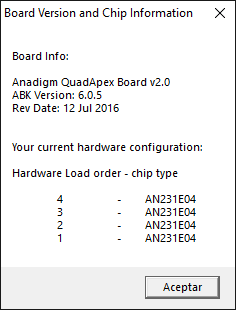
\includegraphics[width = 5cm]{G1_AD2_board_info.png}
	\end{figure}
	
	La Figura \ref{fig:G1_AD2_board_info} muestra la información que despliega AD2 acerca de la tarjeta donde todas las 4 FPAA están configuradas en cadena. Si menos FPAA están configuradas entonces la información de la placa mostrará cuantas FPAA están disponibles.

	Ahora debería ser posible descargar un circuito desde AD2. Para hacer esto simplemente es necesario dar clic sobre el icono de descarga (a la izquierda del signo de interrogación amarillo, debajo de Dynamic Config). Como alternativa presionar Ctrl + W. Un LED amarillo comenzará a parpadear y un sonido de campanilla se escuchará mientras cada FPAA es configurada, finamente un LED verde se encenderá indicando que todas las FPAA han sido configuradas correctamente. Un LED rojo indicará que la configuración falló. Es importante que el número de FPPA en AD2 coincida con el número de FPAA habilitadas en la placa. Por ejemplo, si la tarjeta fue configurada con una cadena de 3 FPAA, entonces estará esperando 3 configuraciones de FPAA para ser descargadas desde AD2 de lo contrario podrían ocurrir errores.
	
	
		\subsection{Configuración de relojes}
	
	Las configuraciones de los CAMs dependen de las frecuencias de reloj que se seleccionen para cada FPAA. Cada FPAA tiene dos fuentes de frecuencias de reloj de sistema \textbf{Sys1} y \textbf{Sys2}, y seis frecuencias de reloj de chip, desde \textbf{Clock 0} hasta \textbf{Clock 5} que son subdivisiones de cualquiera de las fuentes de reloj sistema. Seleccionar y configurar correctamente los relojes es importante ya que el rango de operación de los CAMs depende de esto.  En la Figura \ref{fig:G3_Frecuencias_AD2} se muestra la ventana de configuración de frecuencias de reloj.
	
	\begin{figure}[!hbp] 
		\caption{Ventana de configuración de frecuencias de reloj en AD2.}
		\label{fig:G3_Frecuencias_AD2}
		\centering
		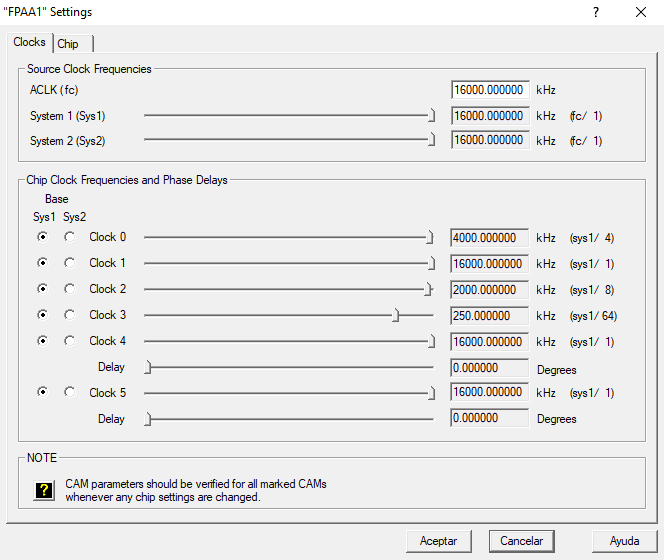
\includegraphics[width = 12cm]{G3_Frecuencias_AD2.png}
	\end{figure}

	La tarjeta tiene una fuente de frecuencia de reloj principal llamada \textbf{ACLK} o $f_{c}$ cuya frecuencia es igual a $16$ MHz y a pesar de que es posible modificarla se recomienda no hacerlo. Sys1 y Sys2 dependen de esta frecuencia y pueden ser modificadas utilizando las siguientes ecuaciones:

	\begin{equation}
		\mathrm{Sys1} = \frac{f_{c}}{m} \qquad \mathrm{Sys2} = \frac{f_{c}}{m}
		\label{ec:sys_clock}
	\end{equation}
	donde $m\in [1,510]$ y es par. Usualmente Sys1 y Sys2 no se modifican drásticamente y $m$ se mantiene en valores pequeños sin embargo es necesario entender que estas dos fuentes de frecuencias de reloj a su vez controlan a las fuentes de reloj de chip desde Clock 0 hasta Clock 5 dada la siguiente ecuación:

	\begin{equation}
		\mathrm{Clock\,} h = \frac{\mathrm{Sys1}}{n}	\qquad   \mathrm{Clock\,} h = \frac{\mathrm{Sys2}}{n}
		\label{ec:clock_h}
	\end{equation}
	donde $n\in[1,510]$ y es par y $h\in[0,5]$. Configurar las fuentes de reloj de chip cobrará importancia en secciones posteriores y las ecuaciones deben tenerse presentes.

	\section{NI ELVIS II+}

		\subsection{¿Qué es la NI ELVIS II+?}
	El NI Engineering Laboratory Virtual Instrumentation Suite (NI ELVIS) es un dispositivo modular de laboratorio educativo de ingeniería que incluye un osciloscopio, multímetro digital, generador de funciones, fuente de alimentación variable, \textbf{analizador de Bode} y otros instrumentos comunes de laboratorio. Es necesario utilizar una PC en conjunto con la NI ELVIS para acceder a todas sus prestaciones y la comunicación entre las dos se hace vía USB.

		\subsection{Instalación}

	El NI ELVIS II+ requiere del software NI ELVISmx para su correcto funcionamiento, actualmente se encuentra en la versión 19.0 sin embargo la versión 16.0 posee mayor compatibilidad y es la que se recomienda instalar. El software se puede encontrar dirigiéndose al siguiente link:  

	\begin{center}
		\url{https://www.ni.com/es-mx/support/downloads/drivers/download.ni-elvismx.html}
	\end{center}
	la instalación es directa y basta con leer cuidadosamente las ventanas emergentes para no cometer errores.
		
		\subsection{Puesta en marcha y calibración}

	Una vez terminada la instalación del software, para poner en marcha el NI ELVIS es necesario seguir los siguientes pasos:
	\begin{enumerate}
		\item Realizar las conexiones que se muestran en la Figura \ref{fig:T15_ELVIS_3} las cuales consisten en conectar un cable USB entre la computadora y el NI ELVIS, conectar la fuente de alimentación al NI ELVIS y al toma corriente.
		\item Activar el switch de alimentación principal, ver Figura \ref{fig:T13_ELVIS}, los leds indicadores ACTIVE y READY se iluminarán, esperar hasta que quede solo encendido el segundo. Automáticamente se abrirá el programa NI ELVISmx Intrument Laucher.
		\item Activar el switch de alimentación de la placa de prototipado, ver Figura \ref{fig:T13_ELVIS}, el led indicador POWER se iluminará.
		\item En la ventana NI ELVISmx Intrument Laucher dar clic en la opción Resources y después en Measurement and Automation Explorer, de desplegará una nueva ventana, en ella dar clic en la siguiente ruta My System/Devices and Interfaces/NI ELVIS II+``Dev1''. Dar clic en Reset y en Self-Test para comprobar la comunicación y después dar clic en Self-Calibrate. Una vez terminada la calibración no es necesario mantener la ventana de la calibración abierta.
	\end{enumerate}		
	
	
	\begin{figure}[!ht]
		\begin{minipage}[c]{0.65\textwidth}
			\begin{center}
				\caption{Diagrama de conexiones de NI ELVIS II+.}
				\label{fig:T15_ELVIS_3}
				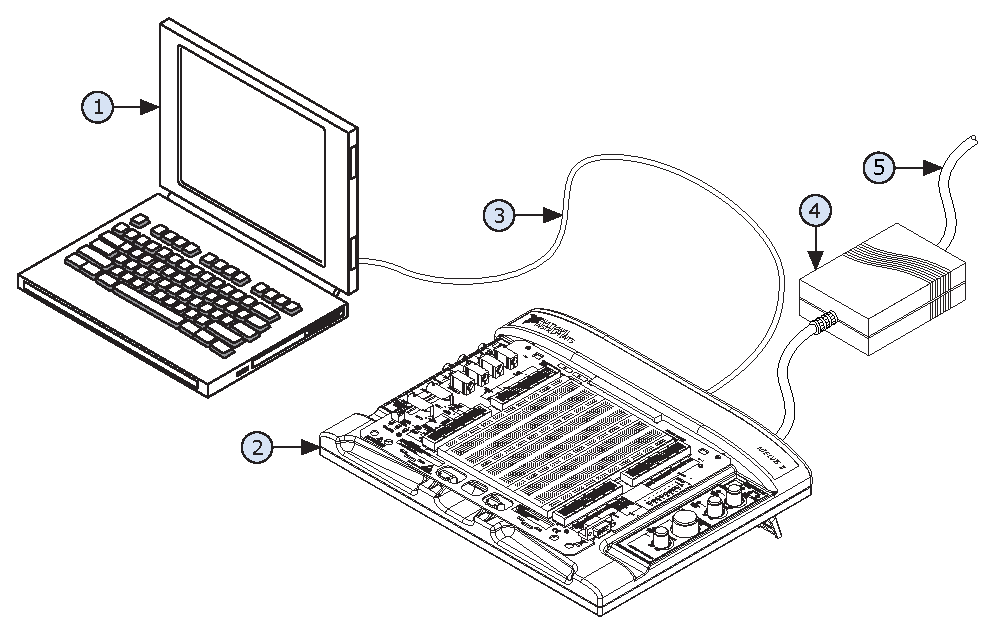
\includegraphics[width = 10cm]{T15_ELVIS_3.eps}
			\end{center}
		\end{minipage} \hfill \begin{minipage}[c]{0.3\textwidth}
			\begin{enumerate}
		  		\item Laptop.
				\item Cable USB.
				\item Fuente de alimentación AC/DC.
				\item Al tomacorriente.
			\end{enumerate}
		\end{minipage}
	\end{figure}
	
	
	\begin{figure}[!ht]
		\begin{minipage}[c]{0.65\textwidth}
			\begin{center}
				\caption{Puestos y switches de NI ELVIS II+.}
				\label{fig:T13_ELVIS}
				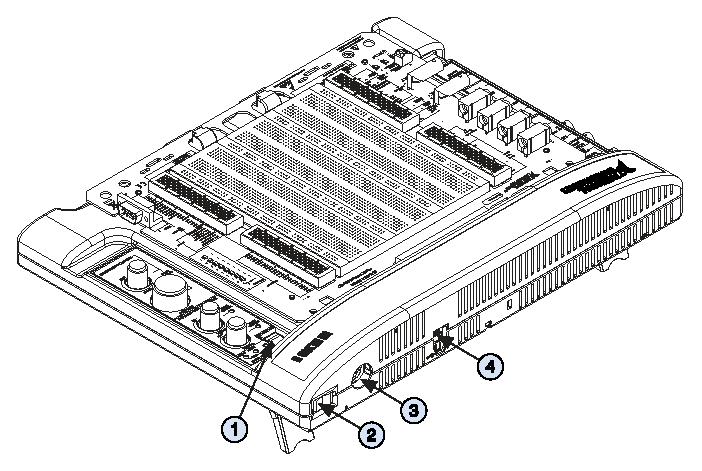
\includegraphics[width = 10cm]{T13_ELVIS.eps}
			\end{center}
		\end{minipage} \hfill \begin{minipage}[c]{0.3\textwidth}
			\begin{enumerate}
		  		\item Switch de alimentación de placa de prototipado.
				\item Switch de alimentación principal.
				\item Conector de alimentación AC/DC.
				\item Conector USB.
			\end{enumerate}
		\end{minipage}
	\end{figure}
	
	Los pasos anteriores se tienen que repetir siempre que se comience a trabajar con la NI ELVIS II+.
	
		\subsection{Diagramas de Bode}\label{sec:diagrama_de_bode}
		
	El diagrama de Bode que se obtiene del NI ELVIS II+ se hace por medio de un barrido en frecuencia real. El dispositivo genera una señal estímulo senoidal de 1V de amplitud desde una frecuencia inicial hasta una frecuencia final con un paso definido por el usuario, esta señal se introduce a la entrada de circuito a analizar y utilizando dos puntas de osciloscopio se mide tanto el estímulo como la respuesta del circuito a este. 
	
	Para poder realizar un diagramas de Bode utilizando el NI ELVIS II+ es necesario seguir la siguiente metodología:
		
		\begin{enumerate}
			\item Realizar la calibración descrita en la sección anterior.
			\item Construir el circuito a analizar en la placa de prototipado de la NI ELVIS II+ y alimentarlo con las fuentes de alimentación incluidas en el dispositivo, ver Figura \ref{fig:T14_ELVIS_2_B}, en caso de tratarse de un circuito externo compartir tierras con el dispositivo. 
			\item Conectar la señal FGEN ubicada en la placa de prototipado a la entrada del circuito a analizar y conectar la referencia del circuito a GROUND, ver Figura \ref{fig:T14_ELVIS_2_B}.
			\item Conectar una punta de osciloscopio al conector BNC SCOPE CH 0, este será el canal del estimulo y debe conectarse a la entrada del circuito y a GROUND, ver Figuras \ref{fig:T14_ELVIS_2_A} y \ref{fig:T14_ELVIS_2_B}.
			\item Conectar una punta de osciloscopio al conector BNC SCOPE CH 1, este será el canal de la respuesta y debe conectarse a la salida del circuito y a GROUND, ver Figuras \ref{fig:T14_ELVIS_2_A} y \ref{fig:T14_ELVIS_2_B}.
			\item Abrir la aplicación Bode Analyzer.
			\item Realizar las siguientes configuraciones:
				\begin{multicols}{2}
				    \begin{enumerate}
				    	\item Stimulus Channel: SCOPE CH 0
						\item Response Channel: SCOPE CH 1 
						\item Start Frequency:	100 Hz
						\item Stop Frequency:	10 kHz
						\item Steps:			10 (per decade)
						\item Peak Amplitudde:	1 V
						\item Op-Amp Signal Polarity: Normal
						\item Mapping:			Logarithmic
						%\item[\vspace{\fill}]
				    \end{enumerate}
			    \end{multicols}
		    \item Iniciar la medición del diagrama de Bode dando clic en Run.
		    \item Para guardar los datos obtenidos dar clic en Log y seleccionar una ruta de destino.
		\end{enumerate}
	
	\begin{figure}[!ht]
		\begin{minipage}[c]{0.65\textwidth}
			\begin{center}
				\caption{Puestos BNC de osciloscopio de NI ELVIS II+.}
				\label{fig:T14_ELVIS_2_A}
				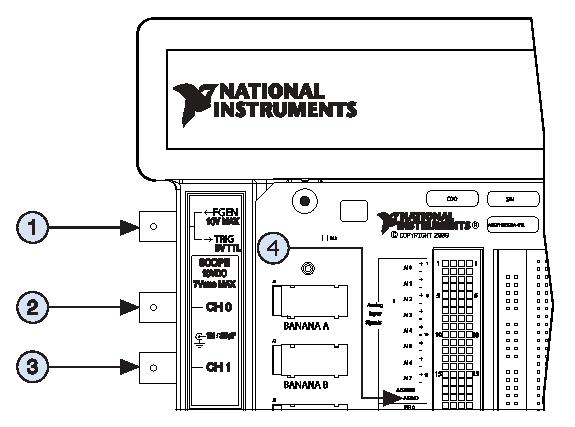
\includegraphics[width = 10cm]{T14_ELVIS_2_A.eps}
			\end{center}
		\end{minipage} \hfill \begin{minipage}[c]{0.3\textwidth}
			\begin{enumerate}
		  		\item Conector BNC FGEN de salida de generador de funciones.
				\item Conector BNC SCOPE CH 0.
				\item Conector BNC SCOPE CH 1.
				\item Señal AIGND ubicada en la placa de prototipado.
			\end{enumerate}
		\end{minipage}
	\end{figure}
	
	\begin{figure}[!ht]
		\begin{minipage}[c]{0.65\textwidth}
			\begin{center}
				\caption{Fuentes de alimentación en NI ELVIS II+ y FGEN.}
				\label{fig:T14_ELVIS_2_B}
				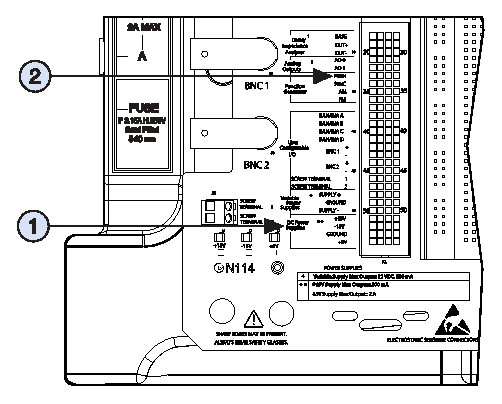
\includegraphics[width = 9cm]{T14_ELVIS_2_B.eps}
			\end{center}
		\end{minipage} \hfill \begin{minipage}[c]{0.3\textwidth}
			\begin{enumerate}
		  		\item Alimentaciones en placa de prototipado. Pines $\pm$15V, +5V y GROUND.
		  		\item Señal FGEN ubicada en la placa de prototipado.
			\end{enumerate}
		\end{minipage}
	\end{figure}
	
		\subsection{Ejemplo práctico}
	Como ejemplo consideremos un filtro pasabajas activo el cual posee la siguiente función de transferencia:
	
	\begin{equation}
		T(s) = - \frac{k \omega_{0}}{s + \omega_{0}}
		\label{ec:pasabajas_TF}
	\end{equation}
	donde:
	\begin{equation}
		\omega_{0} = \frac{1}{R_{f} C} \qquad k = \frac{R_{f}}{R_{i}}
	\end{equation}
	si consideramos los valores $R_{f} = R_{i}= 8.2$k$\Omega$ y $C = 1$uF entonces la función de transferencia (\ref{ec:pasabajas_TF}) se reescribe como:
	
	\begin{equation}
		T(s) = - \frac{1.22 \cdot 10^{5}}{s + 1.22 \cdot 10^{5}}
	\end{equation}
	donde $\omega_{0} = 1.22 \cdot 10^{5} $ y $k = 1$. En la Figura \ref{fig:V8_pasabajas_activo} se muestra el diagrama esquemático del filtro pasabajas activo.
	
	\begin{figure}[hbtp]
		\caption{Diagrama esquemático de filtro pasabajas activo.}
		\label{fig:V8_pasabajas_activo}
		\centering
		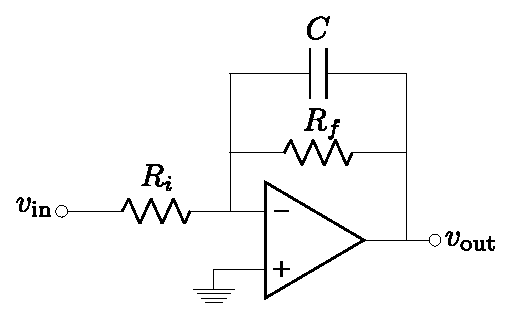
\includegraphics[width = 6.5cm]{V8_pasabajas_activo.eps}
	\end{figure}
	
	Utilizando LTspice se puede hacer la simulación de respuesta en frecuencia del circuito utilizando el modelo spice del amplificador operacional TL081 que se puede encontrar en el siguiente link:
	
	\begin{center}
		\url{http://www.ti.com/lit/zip/sloj069}
	\end{center}
	un código en spice se muestra en el apéndice \ref{cod:LTspice_simulacion} el cual realiza un barrido en frecuencia desde 1 kHz hasta 10 MHz con una resolución de 1000 puntos por década. Una vez realizada la simulación se exportan los resultados de magnitud y fase en archivo de texto para su manipulación en Matlab.
	
	Utilizando la metodología descrita en la sección anterior considerando las siguientes configuraciones:
	\begin{multicols}{2}
	    \begin{enumerate}[label=\alph*.]
	    	\item Stimulus Channel: SCOPE CH 0
			\item Response Channel: SCOPE CH 1 
			\item Start Frequency:	1000 Hz
			\item Stop Frequency:	5 MHz
			\item Steps:			20 (per decade)
			\item Peak Amplitudde:	1 V
			\item Op-Amp Signal Polarity: Normal
			\item Mapping:			Logarithmic
			%\item[\vspace{\fill}]
	    \end{enumerate}
	\end{multicols}
	\noindent
	se obtiene el diagrama de Bode experimental del circuito pasabajas activo como se muestra en la Figura \ref{fig:V9_elvis_pasabajas}. Al igual que con la simulación se exportan los resultados en un archivo de texto.
	
	Finalmente en el apéndice \ref{cod:diagramas_bode_comparativos} se muestra un código para cargar los datos tanto de la simulación como experimentales y compararlos con la respuesta ideal. El código genera la gráfica de la Figura \ref{fig:V10_bodes_comparativos}. 
	
	\begin{figure}[h!]
		\caption{Diagrama de Bode experimental utilizando el NI ELVIS II+.}
		\label{fig:V9_elvis_pasabajas}
		\centering
		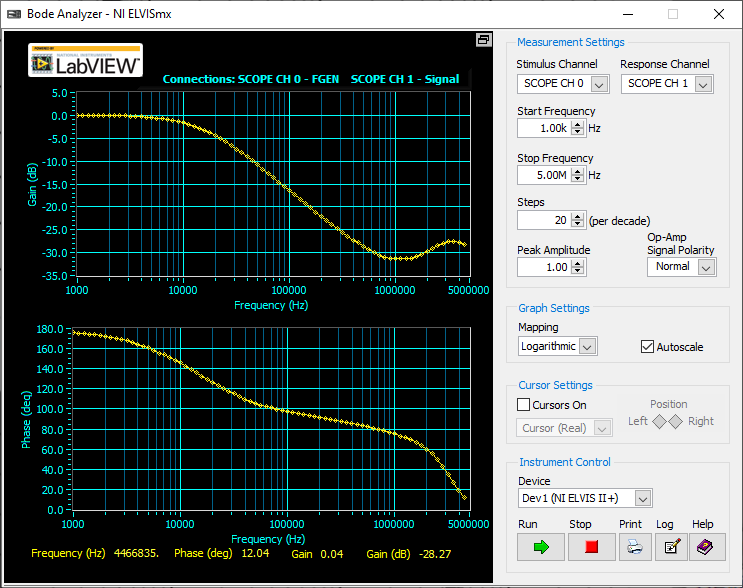
\includegraphics[width = 10cm]{V9_elvis_pasabajas.png}
	\end{figure}
	
	\begin{figure}[h!]
		\caption{Diagramas de Bode comparativos, respuesta ideal, simulación y experimental.}
		\label{fig:V10_bodes_comparativos}
		\centering
		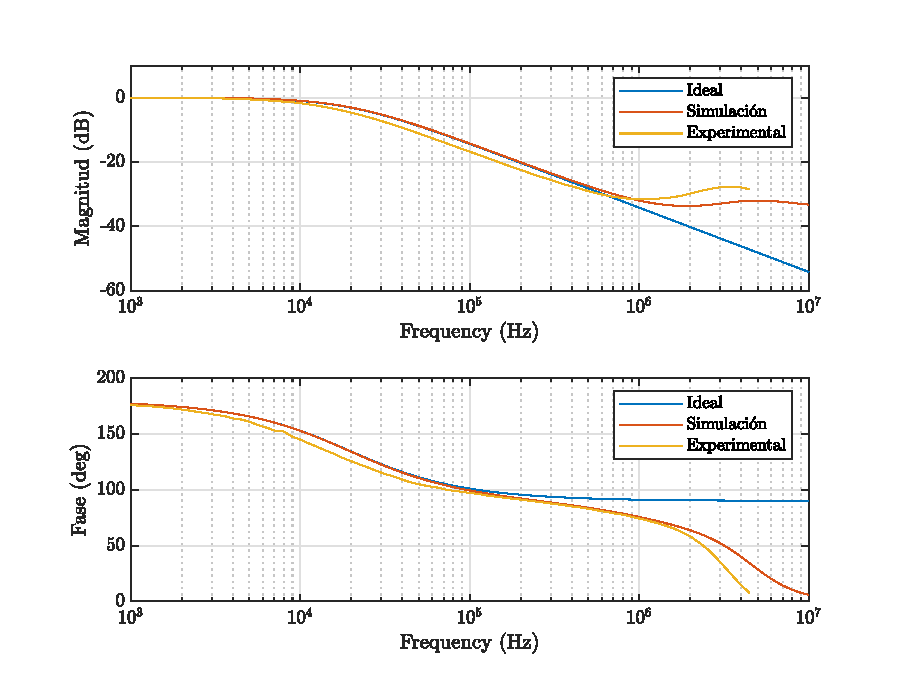
\includegraphics[width = 12cm]{V10_bodes_comparativos.eps}
	\end{figure}
	Los resultados experimentales coinciden casi a la perfección con la simulación . En frecuencias arriba de 1 MHz la respuesta se aleja del comportamiento ideal debido a las limitaciones a altas frecuencias del TL081.
	
	\section{Implementación con aproximación de primer orden}
	
		\subsection{Filtro bilineal configuración polo y cero}
	
	Para realizar la implementación física de la aproximación de primer orden del integrador fraccionario se utilizó el CAM \textbf{FilterBilinear} en su modo \textbf{Pole and Zero}, esto debido a su flexibilidad y semejanza con la función de transferencia de la aproximación de la CFE de primer orden. La función de transferencia del CAM en este modo es la siguiente:
	
	\begin{equation}
		\frac{V_{\mathrm{out}} (s)}{V_{\mathrm{in}}(s)} = -\frac{G_{H} (s + 2 \pi f_{z})}{s + 2 \pi f_{p}}
		\label{ec:CAM_bilineal}
	\end{equation}
	donde $G_{L}$ esta definida como:
	\begin{equation}
		G_{L} = \frac{f_{z}}{f_{p}} G_{H}
	\end{equation}
	y donde $G_{L}$ es la ganancia en DC, $G_{H}$ es la ganancia de alta frecuencia, $f_{p}$ es la frecuencia del polo y $f_{z}$ es la frecuencia del cero. Si se utiliza un CAM de ganancia inversora (\textbf{GainInv}) se puede prescindir del signo negativo de la ecuación (\ref{ec:CAM_bilineal}).
	
	La función de transferencia de la aproximación con la CFE de primer orden, como se mencionó anteriormente es la siguiente:
	\begin{equation}
		\genfrac{}{}{0pt}{0}{}{_{(c_{2})}} \frac{1}{s^{\alpha}} \approx \frac{(1 - \alpha)s + (1 + \alpha) }{(1 + \alpha)s + (1 - \alpha)} 
		\label{ec:cfe_primer_orden}
	\end{equation}
	si consideramos la siguiente sustitución:
	\begin{equation}
		A = \frac{1 - \alpha}{1 + \alpha}
	\end{equation}
	podemos reescribir la ecuación (\ref{ec:cfe_primer_orden}) de la siguiente manera:
	\begin{equation}
		\genfrac{}{}{0pt}{0}{}{_{(c_{2})}} \frac{1}{s^{\alpha}} \approx \frac{A s + 1}{s + A}
		\label{ec:cfe_primer_orden_simp}
	\end{equation}
	no obstante el ancho de bando de la ecuación (\ref{ec:cfe_primer_orden_simp}) es de $10^{-1}$ rad/s hasta $10^{1}$ rad/s, ver Figura \ref{fig:F10_bode_escalamiento}, lo cual es un rango de frecuencias muy bajo y presenta dificultades en su implementación. Por  esta razón se opta por aplicar un escalamiento en frecuencia a la ecuación (\ref{ec:cfe_primer_orden_simp}) utilizando los siguiente pasos: 
	
	\begin{enumerate}
		\item Cambiamos la variable compleja por $p$ la cual representa la frecuencia actual:
			\begin{equation}
				N(p) =  \frac{A p + 1}{p + A}
			\end{equation}
		\item Utilizamos la sustitución $p = \cfrac{s}{k_{f}}$:
			\begin{equation}
				N(s) =  \frac{A s k_{f}^{-1} + 1}{s k_{f}^{-1} + A}
			\end{equation}
		\item Reescribimos de una manera más conveniente:
			\begin{equation}
				\genfrac{}{}{0pt}{0}{}{_{(c_{2})}} \frac{1}{s^{\alpha}} \approx \frac{A s + k_{f}}{s + A k_{f}}
				\label{ec:cfe_primer_orden_simp_esc}
			\end{equation}
	\end{enumerate}	
		
	El factor de escalamiento $k_{f}$ se puede elegir a conveniencia dependiendo del ancho de banda necesario, no obstante la frecuencia de entrada de la mayoría de los CAM esta limitada aproximadamente a valores menores de 2 MHz, esto debido a que el tipo de procesamiento de señal del CAM se basa en arquitecturas de datos muestreados. Por esta razón se opta por un escalamiento con un factor $k_{f} = 2\pi 1000$. En la Figura \ref{fig:F12_bode_1er_orden_escalado} se muestra el resultado de aplicar el escalamiento. El nuevo ancho de banda abarca desde $100$ Hz hasta $10$ kHz el cual se encuentra dentro del rango de operación de los CAMs.
	
	\begin{figure}[hbtp]
		\caption{Diagrama de bode de ecuación (\ref{ec:cfe_primer_orden_simp_esc}) para un integrador fraccionario con $k_{f} = 2\pi 1000$ y  $\alpha = 0.5$.} 
		\label{fig:F12_bode_1er_orden_escalado}
		\centering
		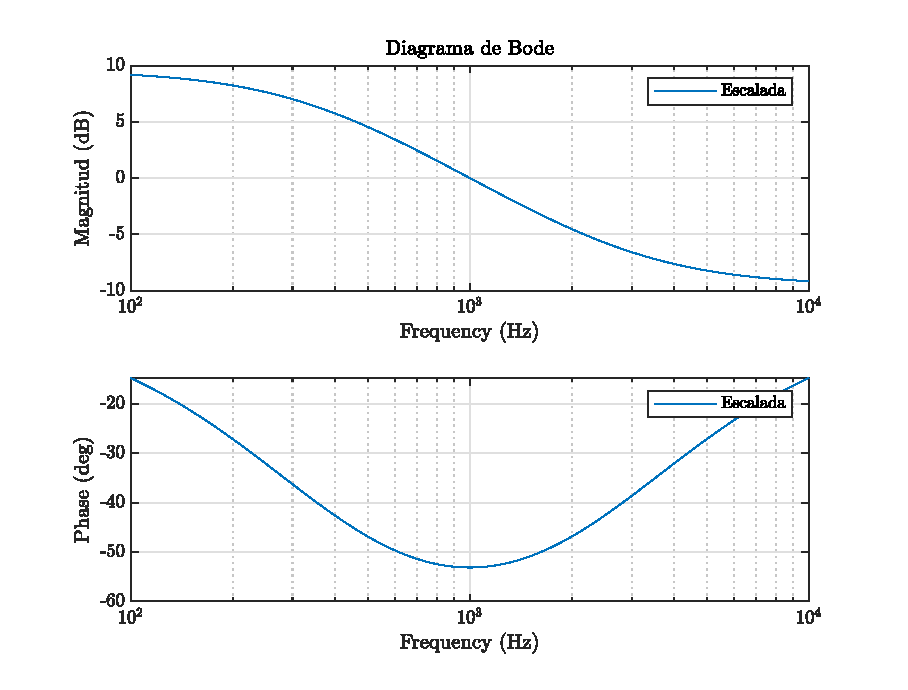
\includegraphics[width=12cm]{F12_bode_1er_orden_escalado.eps}
	\end{figure}
	
	 Para poder configurar el CAM FilterBilinear es necesario encontrar los valores correctos para los parámetros $G_{H}$, $G_{L}$, $f_{z}$ y $f_{p}$ dado un orden $\alpha$, y esto se logra igualando las ecuaciones (\ref{ec:cfe_primer_orden_simp_esc}) y (\ref{ec:CAM_bilineal}) con el fin de encontrar expresiones para calcularlos.
	 
	 \begin{equation}
	 \frac{G_{H}(s + 2 \pi f_{z})}{s + 2 \pi f_{p}} = \frac{As + k_{f}}{s + A k_{f}}
	 \label{ec:igualar_bilineal}
	 \end{equation}
	 de la ecuación (\ref{ec:igualar_bilineal}) se deducen las siguientes ecuaciones:
	 
	 \begin{equation}
		 G_{H} = A
		 \label{ec:bilineal_gh}
	 \end{equation}
	 
	 \begin{equation}
	 	f_{p} = \frac{A k_{f}}{2 \pi}
	 	\label{ec:bilineal_fp}
	 \end{equation}
	 
	 \begin{equation}
		f_{z} = \frac{k_{f}}{ 2A \pi}
		\label{ec:bilineal_fz}
	 \end{equation}
	 
	 \begin{equation}
	 G_{L} = \frac{1}{A}
	 \label{ec:bilineal_gl}
	 \end{equation}
	utilizando las ecuaciones anteriores y considerando $k_{f} = 2 \pi 1000$ obtenemos los datos de la Tabla \ref{tab:calculos_bilineal}, esta tabla se puede generar utilizando el código del apéndice \ref{cod:A10_calculo_valores_FilterBilienar}, sin embargo debido a que el CAM FilterBilinear depende directamente de la frecuencia de reloj que se seleccione en el parámetro \textbf{ClockA} no todos los valores de la tabla pueden ser ingresados, en la ventana de configuración aparecerán marcados en color rojo, por lo tanto  es necesario hacer un análisis de frecuencias para este parámetro. En la ventana de configuración del CAM, ver Figura \ref{fig:G2_FilterBilinear_config}, se pueden ingresar 3 de los 4 parámetros requeridos, el parámetro restante es calculado automáticamente. Por simplicidad se eligió que el parámetro que se calcule automáticamente sea \textbf{DC Gain}. 
	   
	\begin{figure}[!ht] 
		\caption{Ventana de configuración de parámetros FilterBilinear.}
		\label{fig:G2_FilterBilinear_config}
		\centering
		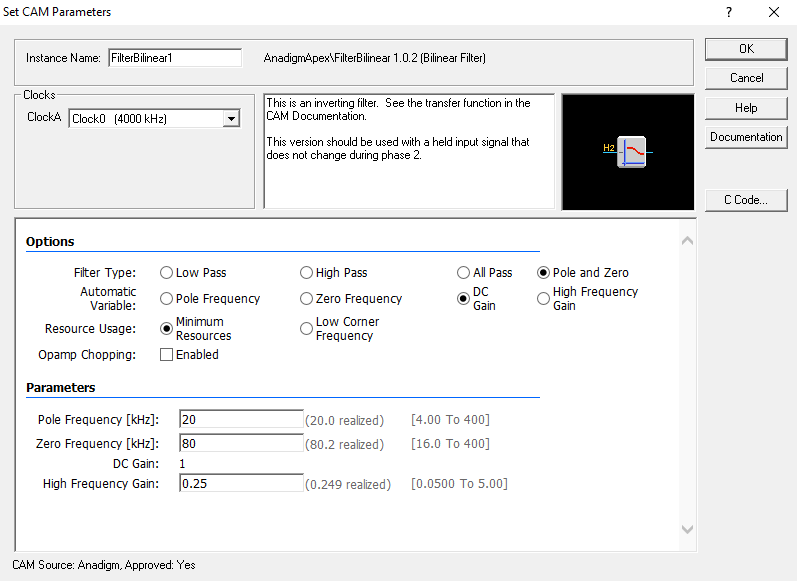
\includegraphics[width = 12cm]{G2_FilterBilinear_config.png}
	\end{figure}

	Los límites absolutos de los valores que se pueden ingresar para las frecuencias $f_{z}$ y $f_{p}$ son $[\frac{F_{c}}{1000}, \frac{F_{c}}{10}]$ donde $F_{c}$ es la frecuencia de reloj que se selecciona para el parámetro \textbf{ClockA} y los límites de ganancia están interrelacionados con los otros parámetros que pueden restringir el rango a menos que el límite absoluto el cual es $\left[0.01 \frac{\mathrm{V}}{\mathrm{V}}, 100.0\frac{\mathrm{V}}{\mathrm{V}} \right]$.  

	\begin{table}[!hbp]                                      
		\centering   
		\caption{Valores para configurar un filtro bilineal como integrador de orden fraccionario en el rango de ordenes de 0.1 a 0.95.}                            
		\label{tab:calculos_bilineal}                                        
			\begin{tabular}{ccccc}                        
			\hline                                              
			$\bm{\alpha}$ & $\bm{f_{p}}\,\,$ [kHz] & $\bm{f_{z}}\,\,$ [kHz] & $\bm{G_{L}}$ & $\bm{G_{H}}$ \\            
			\hline                                              
			0.10 & 0.818182 & 1.222222 & 1.222222 & 0.818182 \\  
			                                              
			0.15 & 0.739130 & 1.352941 & 1.352941 & 0.739130 \\  
			                                            
			0.20 & 0.666667 & 1.500000 & 1.500000 & 0.666667 \\  
			                                              
			0.25 & 0.600000 & 1.666667 & 1.666667 & 0.600000 \\  
			                                              
			0.30 & 0.538462 & 1.857143 & 1.857143 & 0.538462 \\  
			                                              
			0.35 & 0.481481 & 2.076923 & 2.076923 & 0.481481 \\  
			                                              
			0.40 & 0.428571 & 2.333333 & 2.333333 & 0.428571 \\  
			                                            
			0.45 & 0.379310 & 2.636364 & 2.636364 & 0.379310 \\  
			                                             
			0.50 & 0.333333 & 3.000000 & 3.000000 & 0.333333 \\  
			                                             
			0.55 & 0.290323 & 3.444444 & 3.444444 & 0.290323 \\  
			                                             
			0.60 & 0.250000 & 4.000000 & 4.000000 & 0.250000 \\  
			                                              
			0.65 & 0.212121 & 4.714286 & 4.714286 & 0.212121 \\  
			                                             
			0.70 & 0.176471 & 5.666667 & 5.666667 & 0.176471 \\  
			                                              
			0.75 & 0.142857 & 7.000000 & 7.000000 & 0.142857 \\  
			                                              
			0.80 & 0.111111 & 9.000000 & 9.000000 & 0.111111 \\  
			                                             
			0.85 & 0.081081 & 12.333333 & 12.333333 & 0.081081 \\
			                                              
			0.90 & 0.052632 & 19.000000 & 19.000000 & 0.052632 \\
			                                              
			0.95 & 0.025641 & 39.000000 & 39.000000 & 0.025641 \\
			\hline                                              
			\end{tabular}                                                                
	\end{table} 
 
	Hay que tener presente que $F_{c}$ puede ser cualquier Clock, desde el 0 hasta el 5, en otras palabras, $F_{c}$ es igual a la ecuación (\ref{ec:clock_h}). Un análisis de todas las posibles frecuencias para $F_{c}$ dependiente de las subdivisiones dadas por $n$ se muestran en la Tabla \ref{tab:frecuencias_absolutas}. Si se desea ver la tabla completa se puede usar el código del apéndice \ref{cod:A11_rango_de_frecuencias_absolutas_FilterBilinear}. 

	\begin{table}[!hbp]                                      
		\centering   
		\caption{Rango de frecuencias absolutas dependiente de $F_{c}$ y el valor de $n$.}                            
		\label{tab:frecuencias_absolutas}                                        
			\begin{tabular}{cccc}                        
			\hline                                              
			$\bm{F_{c}}\,\,$ [kHz] & $\bm{n}$ & \textbf{min}$\bm{=F_{c} / 1000}\,\,$ [kHz] & \textbf{max}$\bm{=F_{c} /10}\,\,$ [kHz] \\                    
			\hline                                              
			16000.0000 & 1.0000 & 16.0000 & 1600.0000 \\
			                                     
			8000.0000 & 2.0000 & 8.0000 & 800.0000 \\   
			                                     
			4000.0000 & 4.0000 & 4.0000 & 400.0000 \\   
			
			$\vdots$ & $\vdots$ & $\vdots$ & $\vdots$ \\  
			 
			31.6206 & 506.0000 & 0.0316 & 3.1621 \\     
			                                    
			31.4961 & 508.0000 & 0.0315 & 3.1496 \\     
			                                    
			31.3725 & 510.0000 & 0.0314 & 3.1373 \\      
			\hline                                           
			\end{tabular}                                                                
	\end{table} 

	Para demostrar que no todos los valores de la Tabla \ref{tab:calculos_bilineal} pueden ser implementados debido al rango de frecuencias absolutas mostradas en la Tabla \ref{tab:frecuencias_absolutas} consideremos el siguientes ejemplo:

	Imaginemos que queremos implemetar un integrador de orden fraccionario con la aproximación de primer orden, un $\alpha = 0.9$ y escalado en frecuencia para que su ancho de banda se encuentre entre $100$ Hz y $10$ kHz. Dados los requerimientos anteriores $k_{f} = 2 \pi 1000$ y utilizando la Tabla \ref{tab:calculos_bilineal} sabemos que $f_{p} = 0.052632$, $f_{z} = 19.0$, $G_{L} = 19.0$ y $G_{H} = 0.052632$. Como se mencionó anteriormente la fuente de frecuencia de reloj principal $f_{c} = 16$ MHz no debe modificarse y de mismo modo se recomienda que Sys1 y Sys2 tampoco se modifiquen dramáticamente, es decir $m = 1$. Se opta por utilizar el Clock 0 para configurar el CAM FilterBilinear y que este dependa de Sys1 $=16$ MHz. Para que los datos que se ingresen en la ventana de configuración del CAM sean validos estos deben encontrase dentro del rango de frecuencias absolutas de la Tabla \ref{tab:frecuencias_absolutas}, por lo tanto se tiene que elegir un $n$ adecuado de tal manera que $F_{c}$ = Clock 0 = $\frac{\mathrm{Sys1}}{n}$ cumpla con los limites absolutos de frecuencia, en otras palabras que los parámetros $f_{z}$ y $f_{p}$ se encuentren dentro del rango $[\frac{F_{c}}{1000}, \frac{F_{c}}{10}]$. El rango de frecuencias en el que nos tenemos que encontrar para poder implemetentar el integrador es $[f_{p},f_{z}] = [0.052632, 19.0]$, no obstante el proceso de encontrar $n$ es muy laborioso debido a que podría haber más de un valor que haga posible que se encuentren dentro del rango, de mismo modo podría ocurrir el caso contrario y ninguna $n$ cumplir. Por esta razón en el apéndice \ref{cod:A12_grafica_analisis_de_frecuencias_FilterBilinear} se muestra un código para resolver este problema, este genera una gráfica, ver Figura \ref{fig:T11_Analisis_de_frecuencias_FilterBilinear}, la cual muestra la relación entre $n$ y el orden $\alpha$, en otras palabra hasta que orden fraccionario podemos implementar dependiendo del valor de $n$.

	\begin{figure}[hbtp]
		\caption{Gráfica de mérito, análisis de orden fraccionario dependiente de $n$ para implementación con CAM BilinearFilter.} 
		\label{fig:T11_Analisis_de_frecuencias_FilterBilinear}
		\centering
		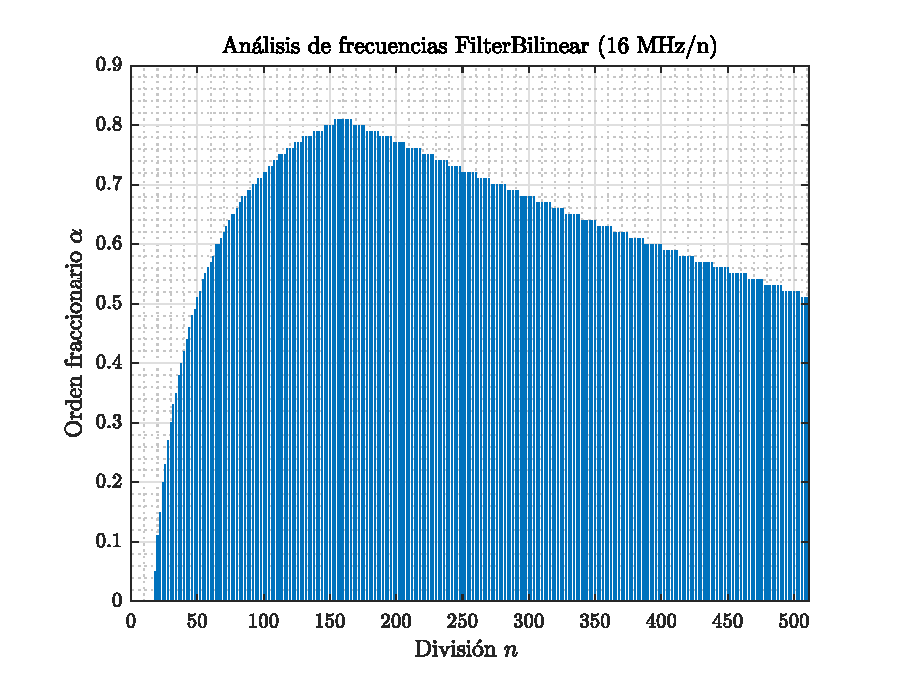
\includegraphics[width=13cm]{T11_Analisis_de_frecuencias_FilterBilinear.eps}
	\end{figure}

	Analizando la Figura \ref{fig:T11_Analisis_de_frecuencias_FilterBilinear} podemos notar que $n = 160$ es el valor con el cual podemos implementar la mayor cantidad de integradores fraccionarios. Haciendo los cálculos Clock 0 = $\frac{16 \mathrm{MHz}}{160} = 100 \mathrm{kHz}$. No obstante únicamente podemos implementar integradores fracciones de orden $\alpha$ dentro del rango $[0.01, 0.81]$. Es importante resaltar que la gráfica de mérito de la Figura \ref{fig:T11_Analisis_de_frecuencias_FilterBilinear} puede cambiar de forma si $k_{f}$ o Sys1 se modifican. Lo anterior es de gran importancia debido a que para diferentes aplicaciones el factor de escalamiento $k_{f}$ puede cambiar y será necesario generar una nueva gráfica de mérito. De mismo modo se puede modificar Sys1 para que la gráfica de mérito se ajuste a las necesidades del diseñador. Utilizando el programa del apéndice \ref{cod:A12_grafica_analisis_de_frecuencias_FilterBilinear} esto no presenta mayor complicación. En la Figura \ref{fig:G4_AD2_BilinearFilter_implementation} se muestra el diagrama de implementación en AnadigmDesigner2, en la Figura \ref{fig:V11_configuracion_relojes} se muestra la configuración de los relojes de la FPAA1 y en la Figura \ref{fig:V12_configuracion_cams} la configuración de los CAM.

	\begin{figure}[!ht] 
		\caption{Implementación de integrador de orden fraccionario utilizando la aproximación de primer orden.}
		\label{fig:G4_AD2_BilinearFilter_implementation}
		\centering
		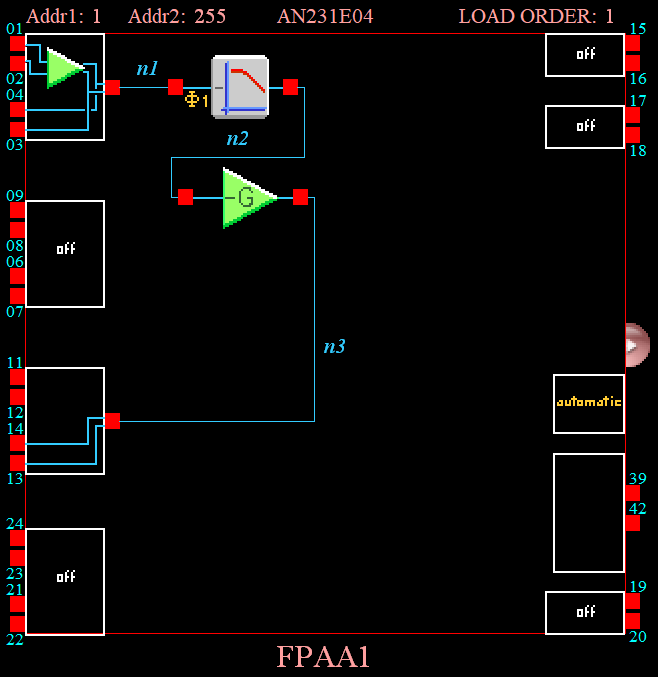
\includegraphics[width = 9cm]{G4_AD2_BilinearFilter_implementation.png}
	\end{figure}
	
	\begin{figure}[!ht] 
		\caption{Configuración de Clocks: FPAA1 con aproximación de primer orden.}
		\label{fig:V11_configuracion_relojes}
		\centering
		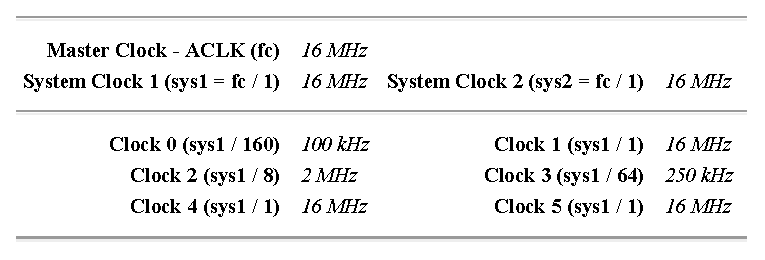
\includegraphics[width = 12cm]{V11_configuracion_relojes.eps}
	\end{figure}
	
	\begin{figure}[!ht] 
		\caption{Configuración de los CAM con aproximación de primer orden.}
		\label{fig:V12_configuracion_cams}
		\centering
		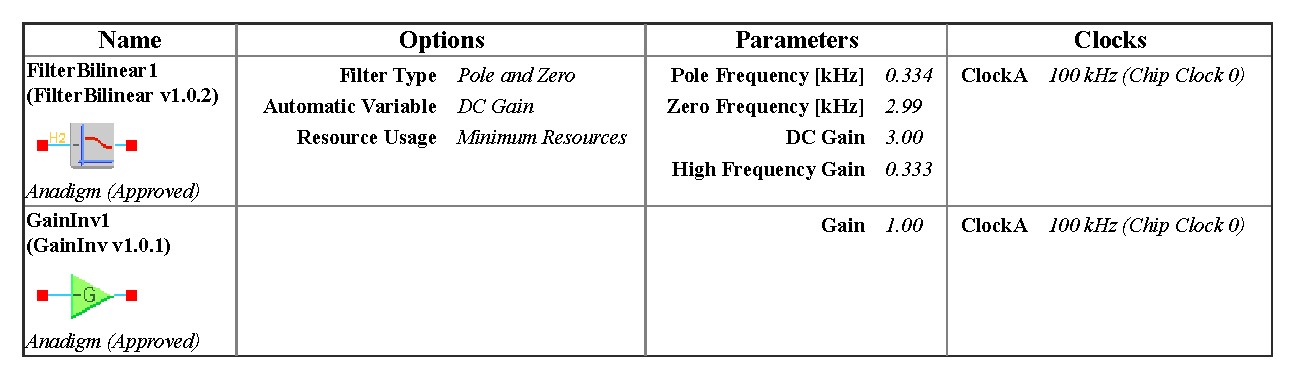
\includegraphics[width = 14cm]{V12_configuracion_cams.eps}
	\end{figure}
	
	Utilizando la NI ELVIS II+ y la metodología descrita en la sección \ref{sec:diagrama_de_bode} se obtiene el diagrama de Bode de la Figura \ref{fig:M1_05}. La respuesta en frecuencia experimental obtenida es casi idéntica a la respuesta teórica, en la Figura \ref{fig:V13_comparacion_exp} se muestran los dos diagramas de Bode juntos para comparación.
	
	
	\begin{figure}[!ht] 
		\caption{Resultados experimentales de respuesta en frecuencia con $\alpha = 0.5$.}
		\label{fig:M1_05}
		\centering
		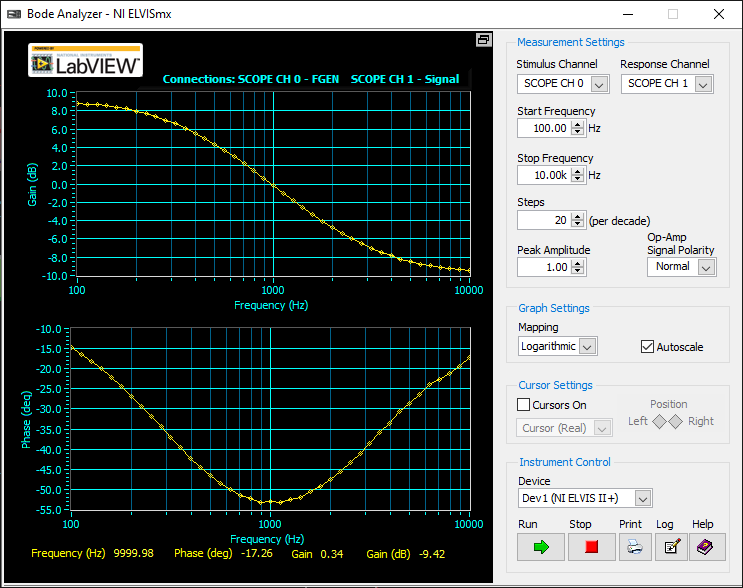
\includegraphics[width = 10cm]{M1_05.png}
	\end{figure}
	
	Es importante tener en cuenta que los limites de voltaje con los que trabaja la tarjeta son $\pm 3$V de modo que al realizar la medición experimental no siempre será posible utilizar una señal senoidal de 1V de amplitud. Como ejemplo consideremos un $\alpha = 0.8$ y $k_{f} = 2 \pi 1000$, al hacer un análisis transitorio de la aproximación de primer orden ante una señal de entrada $u = \sin(2 \pi 100 t)$ obtenemos lo mostrado en la Figura \ref{fig:V14_analisis_transitorio}. El voltaje máximo del transitorio es 7.0477V el cual sobrepasa por mucho los limites de voltaje con los que trabaja la tarjeta por lo que al medir la respuesta en frecuencia utilizando la NI ELVIS II+ obtendremos una medición errónea, esto se puede apreciar en la Figura \ref{fig:V15_transitorio_real}, la salida de la tarjeta se satura en aproximadamente 2.7V y esto provoca que el diagrama de Bode medido sea incorrecto. Para solucionar esto existen dos posibilidades, la primera consiste en modificar la señal de entrada de manera que la salida se encuentre dentro de los voltajes de la tarjeta, para el ejemplo anterior, si se elige $u = 0.35\sin(2 \pi 100 t)$ el voltaje máximo a la salida seria de 2.4667V. La segunda consiste en atenuar la salida por software dentro de AD2 para que esta este dentro de los rangos de voltaje permitidos y después por medio de un circuito externo cancelar la atenuación.
	
	\begin{figure}[hbtp]
		\caption{Diagrama de bode de comparativo, respuesta teórica contra experimental,  $k_{f} = 2\pi 1000$ y  $\alpha = 0.5$.} 
		\label{fig:V13_comparacion_exp}
		\centering
		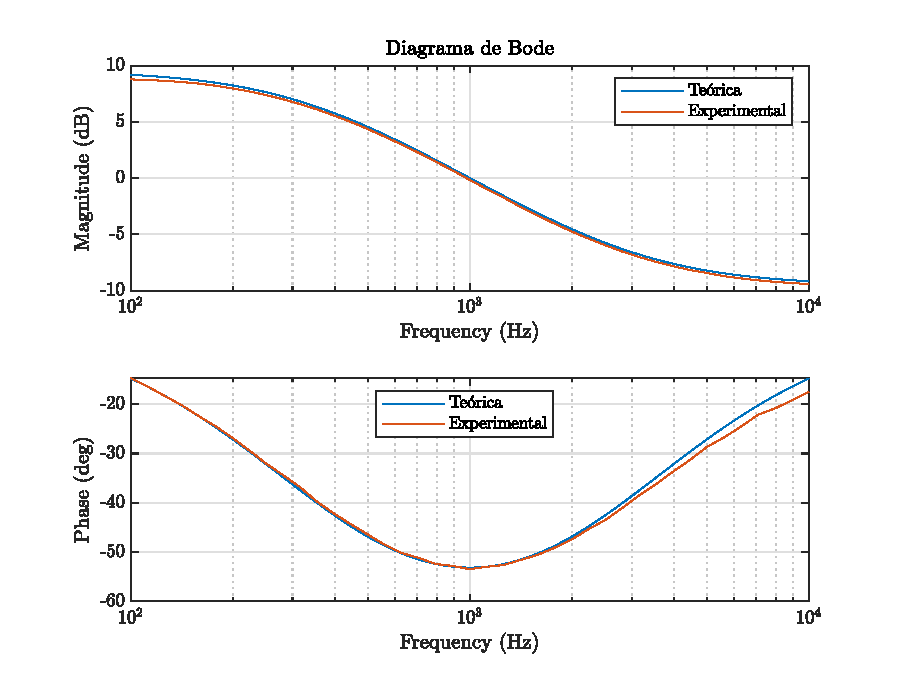
\includegraphics[width=12cm]{V13_comparacion_exp.eps}
	\end{figure}
	
	\begin{figure}[!ht]
		\caption{Análisis transitorio de aproximación de primer orden.} 
		\label{fig:V14_analisis_transitorio}
		\centering
		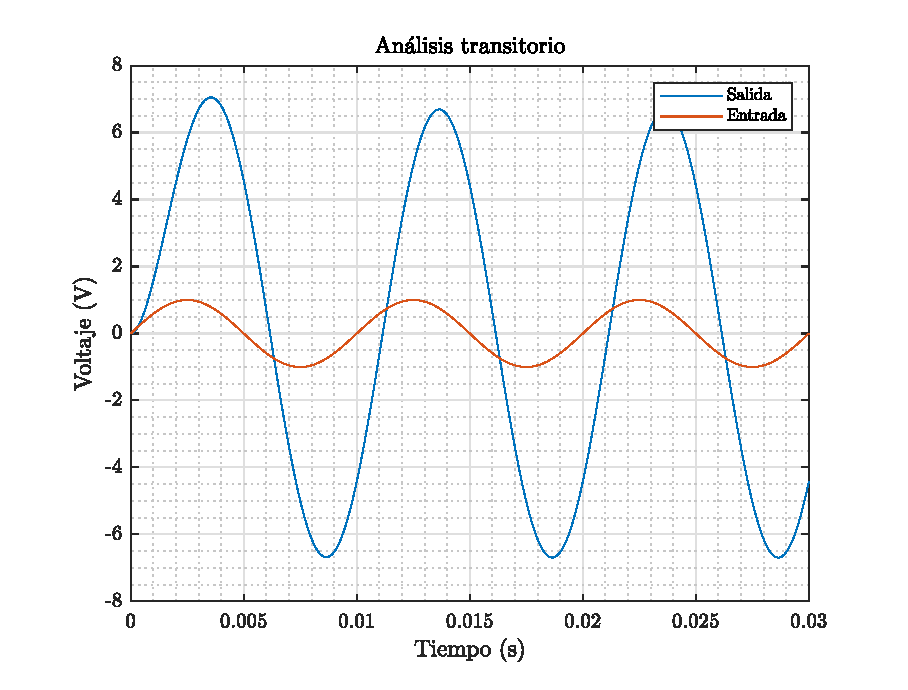
\includegraphics[width=11cm]{V14_analisis_transitorio.eps}
	\end{figure}
	
	\begin{figure}[!ht]
		\caption{Medición experimental de análisis transitorio.} 
		\label{fig:V15_transitorio_real}
		\centering
		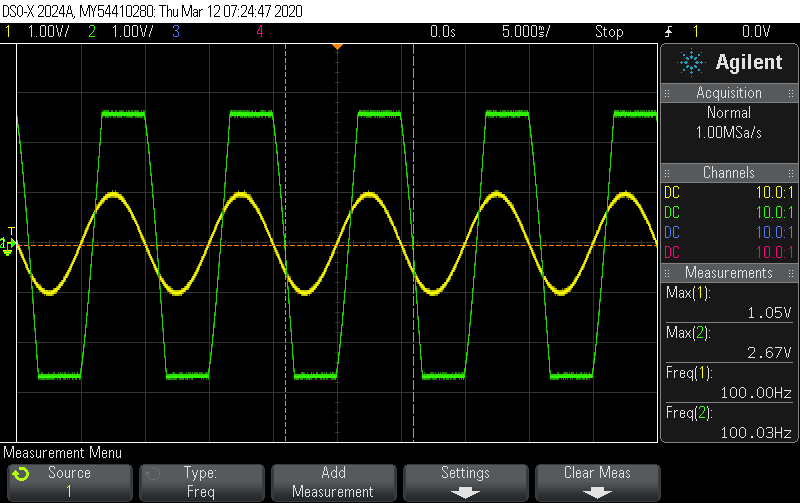
\includegraphics[width=10cm]{V15_transitorio_real.png}
	\end{figure}

		\subsection{Filtro bilineal configuración pasabajas y pasaaltas}

	Otra alternativa para implementar el integrador es utilizando la combinación de un filtro pasaltas y pasabajas y un punto suma. Esto se puede lograr utilizando dos CAM \textbf{FilterBilinear} en su modo \textbf{Low Pass} y \textbf{High Pass} y un CAM \textbf{SumInv} para realizar la suma. La función de transferencia del CAM en el modo pasabajas es la siguiente:
	
	\begin{equation}
		\frac{V_{\mathrm{out}} (s)}{V_{\mathrm{in}}(s)} =  \pm \frac{2 \pi f_{0} G_{1}}{s + 2 \pi f_{0}}
		\label{ec:CAM_bilinear_pasabajas}
	\end{equation}
	y la función de transferencia del CAM en el modo pasaaltas es la siguiente:
	\begin{equation}
		\frac{V_{\mathrm{out}} (s)}{V_{\mathrm{in}}(s)} =  - \frac{ G_{2} s}{s + 2 \pi f_{0}}
		\label{ec:CAM_bilinear_pasaaltas}
	\end{equation}
	donde $G_{1}$ y $G_{2}$ es la ganancia pasabanda para cada uno de los respectivos filtros y $f_{0}$ es la frecuencia de corte en la cual la ganancia es $-3 + 20 \mathrm{log}_{10}G$. Si consideramos que ambos filtros tienen signo negativo y este se cancela con el CAM de suma, entonces la  función de transferencia resultante es:
	
	\begin{equation}
		\frac{V_{\mathrm{out}} (s)}{V_{\mathrm{in}}(s)} = \frac{2 \pi f_{0} G_{1}}{s + 2 \pi f_{0}} + \frac{ G_{2} s}{s + 2 \pi f_{0}} = \frac{G_{2}s + G_{1}2 \pi f_{0}}{s + 2 \pi f_{0}}
		\label{ec:fun_trans_suma_filtros}
	\end{equation}

	Si igualamos la aproximación de primer orden escalada de la ecuación (\ref{ec:cfe_primer_orden_simp_esc}) con la función de transferencia resultante (\ref{ec:fun_trans_suma_filtros}) obtenemos:
	
	\begin{equation}
		\frac{G_{2}s + G_{1}2 \pi f_{0}}{s + 2 \pi f_{0}} = \frac{As + k_{f}}{s + Ak_{f}}
		\label{ec:igualar_suma_filtros}
	\end{equation}
	de la ecuación (\ref{ec:igualar_suma_filtros}) se deducen las siguientes ecuaciones:
	
	\begin{equation}
		G_{1} = \frac{1}{A}
	\end{equation}	
	
	\begin{equation}
		G_{2} = A
	\end{equation}
	
	\begin{equation}
		f_{0} = \frac{A k_{f}}{2 \pi}
	\end{equation}
	
	Los límites absolutos de los valores que se pueden ingresar para $f_{0}$ son $[\frac{F_{c}}{1000}, \frac{F_{c}}{10}]$. No obstante los límites absolutos de frecuencia también están interrelacionados con el valor de ganancia que puede restringir el rango a menos de sus límites absolutos y viceversa. Si consideramos $k_{f} = 2 \pi 1000$ y utilizando las ecuaciones anteriores obtenemos los datos de la Tabla \ref{tab:calculos_bilineal_suma}, esta tabla se puede generar utilizando el código del apéndice \ref{cod:B10_calculo_valores_suma_filtros}.

	\begin{table}[!hbp]                                      
		\centering   
		\caption{Valores para configurar implementación suma de pasabajas y paaltas de ordenes de 0.1 a 0.95.}                            
		\label{tab:calculos_bilineal_suma}                                        
			\begin{tabular}{cccc}                        
			\hline                                              
			$\bm{\alpha}$ & $\bm{G_{1}}\,\,$ [LP] & $\bm{G_{2}}\,\,$ [HP] & $\bm{f_{0}}\,\,$ [kHz]  \\            
			\hline                                              
			0.10 & 1.222222 & 0.818182 & 0.818182 \\ 
			                                 
			0.15 & 1.352941 & 0.739130 & 0.739130 \\ 
			                                 
			0.20 & 1.500000 & 0.666667 & 0.666667 \\ 
			                                
			0.25 & 1.666667 & 0.600000 & 0.600000 \\ 
			                                  
			0.30 & 1.857143 & 0.538462 & 0.538462 \\ 
			                                  
			0.35 & 2.076923 & 0.481481 & 0.481481 \\ 
			                                  
			0.40 & 2.333333 & 0.428571 & 0.428571 \\ 
			                               
			0.45 & 2.636364 & 0.379310 & 0.379310 \\ 
			                                 
			0.50 & 3.000000 & 0.333333 & 0.333333 \\ 
			                                   
			0.55 & 3.444444 & 0.290323 & 0.290323 \\ 
			                                  
			0.60 & 4.000000 & 0.250000 & 0.250000 \\ 
			                                 
			0.65 & 4.714286 & 0.212121 & 0.212121 \\ 
			                                   
			0.70 & 5.666667 & 0.176471 & 0.176471 \\ 
			                                  
			0.75 & 7.000000 & 0.142857 & 0.142857 \\ 
			                                   
			0.80 & 9.000000 & 0.111111 & 0.111111 \\ 
			                                 
			0.85 & 12.333333 & 0.081081 & 0.081081 \\
			                                  
			0.90 & 19.000000 & 0.052632 & 0.052632 \\
			                                  
			0.95 & 39.000000 & 0.025641 & 0.025641 \\
			\hline                                              
			\end{tabular}                                                                
	\end{table} 

	De manera similar a la aproximación con un solo filtro bilineal no todas los valores de la Tabla \ref{tab:calculos_bilineal_suma} pueden ser implementados y es necesario realizar un análisis de los parámetros $G_{1}$, $G_{2}$ y $f_{0}$ con respecto a $n$. Debido a que las ganancias $G_{1}$ y $G_{2}$ pueden ser obtenidas con relativa libertad debido a que el CAM de suma permite añadir otro nivel de ganancia, el problema principal radica en que $f_{0}$ se encuentre dentro de los limites absolutos de frecuencia. Utilizando el programa del apéndice \ref{cod:B12_grafica_analisis_de_frecuencias_suma_filtros} se puede obtener la gráfica de mérito de la Figura \ref{fig:T12_Analisis_de_frecuencias_suma_de_filtros}. Utilizando esta configuración podemos llegar a implementar un integrador fraccionario con un $\alpha$ de hasta $\alpha = 0.93$. Analizando la gráfica de mérito $n = 442$ es el valor ideal, esto debido a que entre mas grande sea $n$ la frecuencia disminuye y esto podría empobrecer el rendimiento. De mismo modo no hay que perder de vista que de ser necesario los parámetros $k_{f}$ y Sys1 pueden modificarse para generar una nueva gráfica de mérito que se ajuste a las necesidades del diseñador. En la Figura  \ref{fig:V16_AD2_imple_suma_filtros} se muestra el diagrama de implementación en AD2, en la Figura \ref{fig:V17_configuracion_relojes} la configuración de los relojes de la FPAA1 y en la Figura \ref{fig:V17_configuracion_relojes} la configuración de los CAM.
	
	\begin{figure}[hbtp]
		\caption{Gráfica de mérito, análisis de orden fraccionario dependiente de $n$ para implementación con suma de filtros.} 
		\label{fig:T12_Analisis_de_frecuencias_suma_de_filtros}
		\centering
		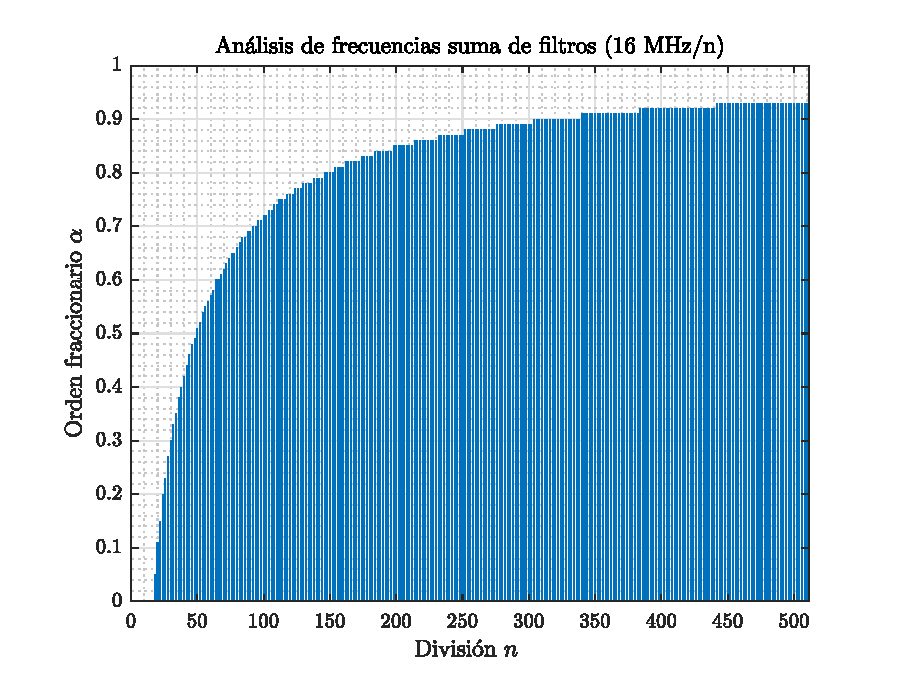
\includegraphics[width=12cm]{T12_Analisis_de_frecuencias_suma_de_filtros.eps}
	\end{figure}
	
	\begin{figure}[!ht] 
		\caption{Implementación de integrador de orden fraccionario utilizando la aproximación de primer orden configuración suma de filtros.}
		\label{fig:V16_AD2_imple_suma_filtros}
		\centering
		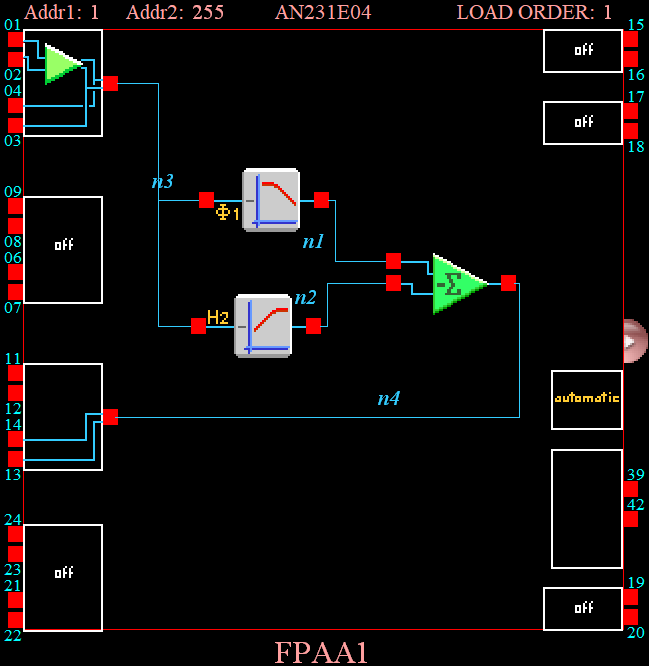
\includegraphics[width = 8.2cm]{V16_AD2_imple_suma_filtros.png}
	\end{figure}
	
	\begin{figure}[!ht] 
		\caption{Configuración de Clocks: FPAA1 con aproximación de primer orden para implementación con suma de filtros.}
		\label{fig:V17_configuracion_relojes}
		\centering
		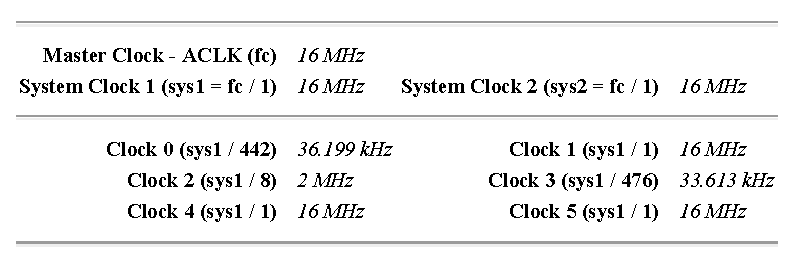
\includegraphics[width = 12cm]{V17_configuracion_relojes.eps}
	\end{figure}
	
	\begin{figure}[!ht] 
		\caption{Configuración de los CAM con aproximación de primer orden para implementación con suma de filtros.}
		\label{fig:V18_configuracion_cams}
		\centering
		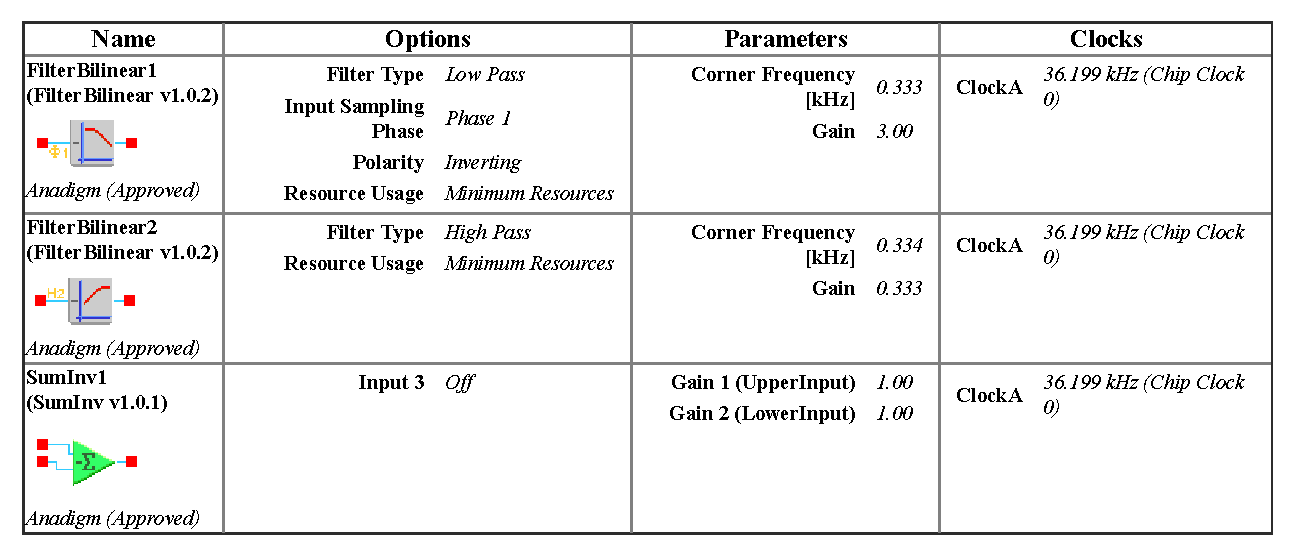
\includegraphics[width = 14cm]{V18_configuracion_cams.eps}
	\end{figure}
	
	Los resultados experimentales de respuesta en frecuencia obtenidos con el NI ELVIS II+ se muestran en la Figura \ref{fig:M2_05} y en la Figura \ref{fig:V15_bodes_comparativos_suma} se muestra la comparación entre la respuesta teórica y la experimental.
	
	La ventaja de utilizar la configuración de suma de dos filtros radica en que aumenta el orden del integrador fraccionario que se puede implementar. Utilizando la configuración polo y cero podemos implementar hasta un $\alpha = 0.81$  mientras que con la suma de dos filtros podemos llegar hasta $\alpha = 0.93$. No obstante analizando las Figuras \ref{fig:V15_bodes_comparativos_suma} y \ref{fig:V13_comparacion_exp} la configuración de suma de filtros presenta ligeramente mayor error que la configuración polo y cero. 
	
	En resumen la configuración de suma filtros requiere mayor cantidad de recursos pero permite implementar un mayor rango de integradores fraccionarios con la desventaja que presenta ligeramente mayor error que la configuración polo y cero. Con la información anterior el diseñador ahora es capaz de elegir entre las dos configuraciones dependiendo de sus necesidades y requerimientos. La tarjeta QuadApex v2.0 como se menciono anteriormente cuenta con 4 FPAAs y administrar los recursos de estas es de vital importancia en el proceso de diseño.
	
	\begin{figure}[!ht] 
		\caption{Resultados experimentales de respuesta en frecuencia con $\alpha = 0.5$ configuración de dos filtros y punto suma.}
		\label{fig:M2_05}
		\centering
		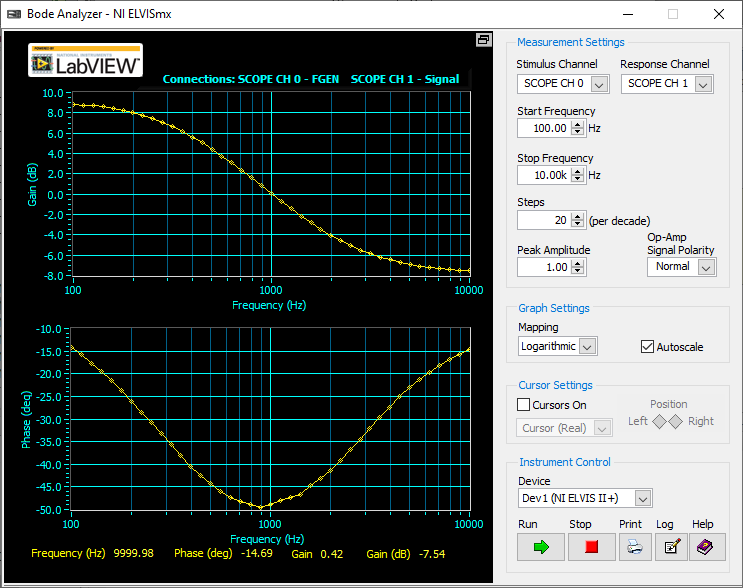
\includegraphics[width = 10cm]{M2_05.png}
	\end{figure}	
	
	\begin{figure}[!ht]
		\caption{Diagrama de bode de comparativo, respuesta teórica contra experimental configuración de dos filtros y punto suma,  $k_{f} = 2\pi 1000$ y  $\alpha = 0.5$.} 
		\label{fig:V15_bodes_comparativos_suma}
		\centering
		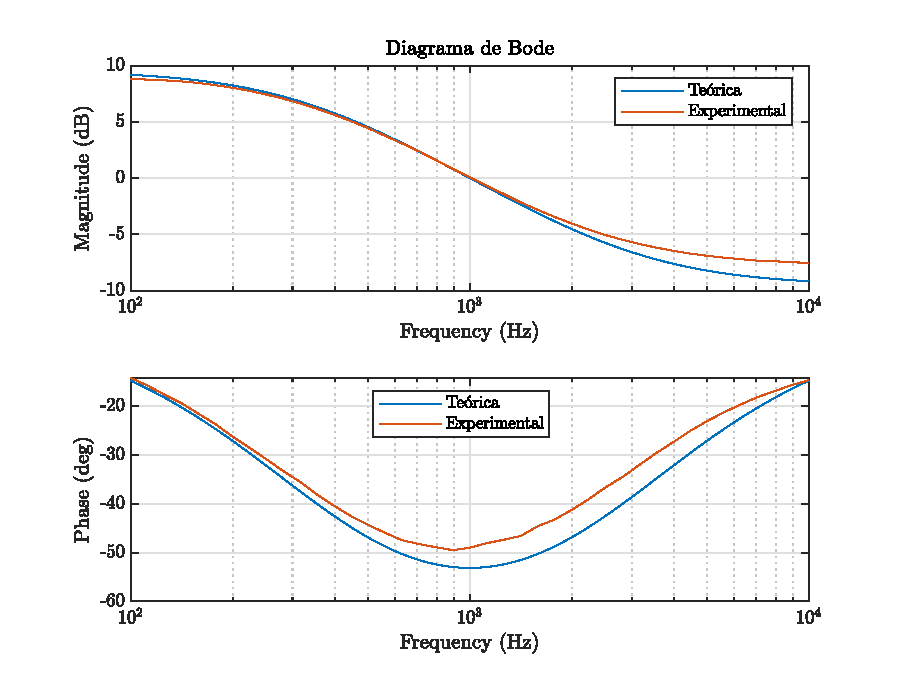
\includegraphics[width=12cm]{V15_bodes_comparativos_suma.eps}
	\end{figure}	

\newpage
	\section{Implementación con aproximación de segundo}
	
	\textbf{FilterBiquad}
	
	\begin{equation}
		\frac{V_{\mathrm{out}} (s)}{V_{\mathrm{in}}(s)} = - \frac{G_{H} \left(  s^{2} + \cfrac{2 \pi f_{z}}{Q_{z}} s + 4 \pi^{2} f_{z}^{2} \right)}{s^{2} + \cfrac{2 \pi f_{p}}{Q_{p}}s + 4\pi^{2} f_{p}^{2} }
	\end{equation}
	donde $G_{L}$  esta definida como:
	
	\begin{equation}
		G_{L} = G_{H} \left( \frac{f_{z}}{f_{p}} \right)^{2}
	\end{equation}
	y donde $G_{L}$ es la ganancia en DC
	
		\begin{equation}
		\genfrac{}{}{0pt}{0}{}{_{(c_{4})}} \frac{1}{s^{\alpha}} \approx \frac{(\alpha^{2} - 3\alpha + 2) s^{2} + (8 - 2 \alpha^{2})s + (\alpha^{2} + 3\alpha + 2) }{(\alpha^{2} + 3\alpha + 2) s^{2} + (8 - 2 \alpha^{2})s + (\alpha^{2} - 3\alpha + 2)}
		\end{equation}
		
		\begin{equation}
			D = \frac{\alpha^{2} - 3 \alpha + 2}{\alpha^{2} + 3\alpha + 2}
		\end{equation}
		
		\begin{equation}
			C = \frac{8 - 2 \alpha^{2}}{\alpha^{2} +  3 \alpha + 2}
		\end{equation}
		
		\begin{equation}
			\genfrac{}{}{0pt}{0}{}{_{(c_{4})}} \frac{1}{s^{\alpha}} \approx = \frac{D s^{2} + Cs + 1}{s^{2} + Cs + D}
		\end{equation}
		
		\begin{equation}
			N(p) = \frac{D p^{2} + Cp + 1}{p^{2} + Cp + D}
		\end{equation}
		
		\begin{equation}
			N(s) = \frac{D (sk_{f}^{-1})^{2} + Csk_{f}^{-1} + 1}{(sk_{f}^{-1})^{2} + Csk_{f}^{-1} + D}
		\end{equation}
		
		\begin{equation}
			N(s) = \frac{D s^{2} + C k_{f}s + k_{f}^{2}}{s^{2} + C k_{f}s + Dk_{f}^{2}}
		\end{equation}
		
		\begin{equation}
			\frac{G_{H} \left(  s^{2} + \cfrac{2 \pi f_{z}}{Q_{z}} s + 4 \pi^{2} f_{z}^{2} \right)}{s^{2} + \cfrac{2 \pi f_{p}}{Q_{p}}s + 4\pi^{2} f_{p}^{2} } = \frac{D s^{2} + C k_{f}s + k_{f}^{2}}{s^{2} + C k_{f}s + Dk_{f}^{2}}
		\end{equation}
		
		
		Hay que notar que hay que cumplir con:
		
		\begin{equation}
			G_{H} \frac{2 \pi f_{z}}{Q_{z}} = \frac{2 \pi f_{p}}{Q_{p}} \quad \Rightarrow \quad  G_{H} \frac{f_{z}}{Q_{z}} = \frac{f_{p}}{Q_{p}}
		\end{equation}
		
		Ecuaciones resultantes metodología 1, todo se calcula utilizando los valores $D$ y $C$, por lo tanto $Q_{z} = Q_{p}$
		
		\begin{equation}
			G_{H} = D
		\end{equation}
		
		\begin{equation}
			f_{z} = \frac{k_{f}}{2 \pi D^{\frac{1}{2}}}
		\end{equation}
		
		\begin{equation}
			f_{p} = \frac{D^{\frac{1}{2}} k_{f}}{2 \pi}
		\end{equation}
		
		\begin{equation}
			Q_{z} = \frac{D^{\frac{1}{2}}}{C}
		\end{equation}
		
		\begin{equation}
			Q_{p} = \frac{D^{\frac{1}{2}}}{C}	
		\end{equation}
		
		\begin{equation}
			G_{L} = \frac{1}{D}
		\end{equation}
		
		Ecuaciones resultantes metodología 2, los factores de calidad $Q_{z}$ y $Q_{p}$ se eligen arbitrariamente  
		
		\begin{equation}
			G_{H} = D
		\end{equation}
		
		\begin{equation}
			f_{z} = \frac{C k_{f} Q_{z}}{D 2 \pi}	
		\end{equation}
		
		\begin{equation}
			f_{p} = \frac{C k_{f} Q_{p}}{ 2 \pi}	
		\end{equation}
		
	Los limites absolutos para los valores que pueden ser ingresados para las frecuencias $f_{z}$ y $f_{p}$ son $[\frac{F_{c}}{500}, \frac{F_{c}}{10}]$. Sin embargo los límites de frecuencia también están interrelacionados con los otros valores de los parámetros, lo que puede restringir el rango a menos de sus límites absolutos. 